\section{Introduction} % The \section*{} command stops section numbering

%\addcontentsline{toc}{section}{Context} % Adds this section to the table of contents
\begin{tcolorbox}[width=\linewidth, colback={boxcolour}]
    \subsection{What is a JSNA?}
    The West Sussex Joint Strategic Needs Assessment (JSNA) sets out the health and wellbeing needs of the population of West Sussex. It is not a single document or piece of analysis but encompasses a range of work, including detailed needs assessments relating to specific subjects or communities, evaluations of new programmes or activities, local surveys, and a range of briefings and ad hoc analyses. {\bf This summary is a brief run-through of the data available.}
\end{tcolorbox}

\paragraph{Scale, Direction and Significance}
Being presented with a lot of facts and figures can be overwhelming. We recommend keeping three things in mind when assessing quantitative data:
\begin{itemize}
    \item Develop a clear understanding of the {\bfseries SCALE} of an issue in understanding population level needs. {\textit For example, in West Sussex there are approximately 160-200 teenage pregnancies in a year.}
    \item Look at the trend or {\bfseries DIRECTION} - if you have a good time series of data, look at the short, medium and long term. {\textit For example, in relation to teenage pregnancy, there is a long downward trend locally and nationally.}
    \item Finally, look at {\bfseries SIGNIFICANCE} - is one year different to the next, or one place compared with another? In this summary we use the term significant to mean \textit{statistically} significant (meaning a difference that isn't due to random chance). \textit{For example, locally there was a rise in teenage pregnancy between 2016 and 2017 but this was small and not significant.}
\end{itemize}

\begin{tcolorbox}[title={CIPFA Neighbours}, colback={boxcolour}]
Data in this summary are compared in a number of ways: over time, between different groups in the population, or by area. We frequently compare information with England and with "comparable local authorities". The Chartered Institute of Public Finance and Accounting (CIPFA) group local authorities by looking at population characteristics (such as population, socioeconomic indicators, household and mortality characteristics).

For West Sussex our current (January 2020) comparable authorities are:
\small
\begin{multicols}{3}
\begin{itemize}
    \item Cambridgeshire
    \item Devon
    \item East Sussex
    \item Essex
    \item Gloucestershire
    \item Hampshire
    \item Kent
    \item North Yorkshire
    \item Northamptonshire
    \item Oxfordshire
    \item Somerset
    \item Staffordshire
    \item Suffolk
    \item Warwickshire
    \item Worcestershire
\end{itemize}
\end{multicols}
\end{tcolorbox}

% \subsection{What's new in the 2021/22 JSNA Summary?}
% \todo[inline]{Given the time now available I might not go through with all these threatened rearrangements of structure}Since the previous West Sussex JSNA Summary (2019/20, available here), Covid-19 has had a profound impact on health care and public health in West Sussex and beyond. Covid-19 at time of writing continues to be a global pandemic with huge implications for public health provision at all levels: locally, nationally and internationally.

% In the years ahead Covid may well change the definition of public health services and what can be expected from them. This is not only because of the disease itself, but also the disruptions to other services that have occurred due to lockdowns and other interventions, and the need to provide additional services to support efforts against covid. 

% As a result, this JSNA summary needs to consider that impact and act as a guide for how and where services need to react to this new world that we live in. At time of writing, it is not known whether the post-Covid world is one in which the disease is all but eliminated or whether it becomes an endemic disease that we must live with. This document aims to support commissioners of services in either eventuality. 

% Previous summaries in West Sussex have structured the document around the life course, broadly grouping topics according to whether they sit with children and young people (starting well), working age adults (living well) and older adults later on in life (ageing well). However, given the need for urgent action in many areas across the life course this chronological sequencing might not be the best method of arranging the topics in question. This summary attempts to define the impact of covid in various areas, categorise them according to current and likely future impact. It then presents these topics in order of urgency. However, the coding of topics across the life course is broadly consistent with previous summaries, as an aid to comparison across years.

% TODO: Possibly cut this section and replace with a Covid focus for this document
\subsection{West Sussex Health and Wellbeing Strategy Priorities 2019-2024}
One of the key functions of the JSNA is to inform the local Health and Wellbeing Strategy. Past JSNA summaries have informed the {\bf West Sussex Health and Wellbeing Strategy 2019-2024}. The Strategy adopts a life course approach. 

Following consultation and wider engagement, the West Sussex Health and Wellbeing Board board identified priorities across three themes - Starting Well, Living and Working Well and Ageing well.

% Contact {\bfseries Aloisia Katsande} (\url{aloisia.katsande@westsussex.gov.uk}) for further information.

\subsubsection{Start Well Priorities}
\begin{itemize}[noitemsep]
    \item Improved mother and baby health and wellbeing, especially for those in most need
    \item Children growing in a safe \& healthy home environment with supporting and nurturing parents and carers
    \item Good mental health for all children
    \item Children and young people leaving care are healthy and independent
\end{itemize}
\subsubsection{Live Well Priorities}
\begin{itemize}[noitemsep]
    \item Individuals, families, friends and communities are connected
    \item People have access to good quality homes providing a secure place to thrive and promote good health, wellbeing and independent living
    \item People are able to look after their own health
    \item People live, work and play in environments that promote health and wellbeing
\end{itemize}

\subsubsection{Age Well Priorities}
\begin{itemize}[noitemsep]
    \item Fewer older people feel lonely or socially isolated
    \item There is a reduction in the number of older people having falls
    \item Older adults stay healthier, happier and independent for longer
    \item People receive good quality end of life care and have a good death
\end{itemize}

Partly in response to the priorities set out in the strategy, we have undertaken some focussed and more detailed analysis including detailing social mobility and multiple deprivation, mental health and wellbeing, emergency admissions, falls, self-care and self-management.

% \subsection{Details of local priorities from the West Sussex Reset Plan}
% The West Sussex corporate plan for 2021-2025 sets put four priorities underpinned by a cross-cutting theme of tackling climate change.
% \todo[inline]{Update to the Covid-19 version of this plan}
% \begin{itemize}[noitemsep]
%     \item Keeping people safe from vulnerable situations
%     \begin{itemize}[noitemsep]
%         \item A timely and proportionate approach to prevention
%         \item Support to people when they need it
%     \end{itemize}
%     \item A sustainable and prosperous economy
%     \begin{itemize}[noitemsep]
%         \item Resetting and rebooting the local economy
%         \item Achieving social value in West Sussex
%         \item Sustainable growth by developing modern infrastructure
%         \item Supporting people to develop the skills they need for the future
%         \item A sustainable economy that adapts to climate change
%         \item Working in partnership
%     \end{itemize}
%     \item Helping people and communities to fulfil their potential
%     \begin{itemize}[noitemsep]
%         \item Access to excellent education and learning
%         \item Tackling inequality
%         \item Promoting and enabling independence
%         \item Safe, connected and cohesive communities
%     \end{itemize}
%     \item Making the best use of resources
%     \begin{itemize}[noitemsep]
%         \item Working together as one council
%         \item Getting the best from our people
%         \item Maximising our income and the productivity of our assets \item Value for money
%         \item Working in partnership
%     \end{itemize}
% \end{itemize}

%------------------------------------------------

\subsection{Impact of Covid-19 on Public Health Outcomes}
The Office of Health inequalities and disparities (OHID) have identified a number of existing Fingertips indicators that can be used to demonstrate the ongoing effects of Covid on population health in West Sussex. Figure~\ref{fig:covid-impacts} shows these indicators and the impact that Covid-19 has had and will continue to have across the life course.

% How do I get the first column labels rotated?
\begin{table*}[]
    \small
    \caption[Impacts of Covid-19 Pandemic across the life course]{Impacts of Covid-19 Pandemic across the life course.}
    \label{fig:covid-impacts}
    \centering
    \begin{tabular}{@{}M{4mm}M{26mm}M{30mm}M{30mm}M{30mm}M{80mm}M{26mm}@{}}
        \toprule
        \ & \textbf{Pregnancy} & \textbf{Infancy} & \textbf{Childhood} & \textbf{Adolescence} & \textbf{Adulthood} & \textbf{Elderly} \\
        \midrule
        \multirow{3}{*}{\rotatebox[origin=c]{270}{Short term}} & Reduced antenatal care & Perinatal mental health & 'Hidden' safeguarding issues & Increased negative health behaviours & Increased negative health behaviours (e.g. substance misuse, alcohol, smoking, gambling, inactivity) & Social isolation and loneliness \\
        \ & Perinatal mental health & Breastfeeding support & Developmental and mental health checks not completed & Deferred sexual health services & Paused commissioned lifestyle services, deferred cancer screening/NHS health checks, reduced health seeking for urgent issues, 'hidden' safeguarding issues & Limited physical activity \\
        \ & \ & Immunisation uptake& Adverse childhood experiences & Low mood and high anxiety & Economic uncertainty & \ \\
        \ & \ & Non-accidental injuries & \ & \  & New anxiety and worsening existing mental illness, PTSD for carers/health workers and families & \ \\
        \cmidrule(r){2-7}
        \multirow{3}{*}{\rotatebox[origin=c]{270}{Medium term}} & Safeguarding risks & Unplanned pregnancies & Adverse childhood experiences & Increased demand for mental health services & Fewer recovering from substance misuse, increased BBV infections, adults smoking, adults overweight/obese & Dementia diagosis \\
        \ & Risky behaviours (Smoking, alcohol, substance misuse) & Admissions for gastrointestinal and respiratory infections & \ & Unwanted pregnancies & Cancer screening coverage (breast, cervical, bowel) and late presentation & Injuries due to falls \\
        \ & \ & Population vaccination coverage reduced and outbreaks&\  & STI diagnoses & Increased demand for grief and bereavement services, employment/training support, claiming out of work benefits & Fuel poverty \\
        \ & \ & \ & \ & \ & People with high anxiety& \ \\
        \cmidrule(r){2-7}
        \multirow{3}{*}{\rotatebox[origin=c]{270}{Long term}} & Low birthweight & Higher risk of poor mental health and physical health & School readiness & Alcohol and substance misuse admissions under 18s & Increased demand for mental health services & Increased morbidity and mortality \\
        \ & Poor attachment & Higher risk of poor social and educational outcomes & \ & Obese children & Under 75s mortality from cardiovascular and liver disease and cancer & \ \\
        \ & Admissions for deliberate or intentional harm & \ & \ & Admissions for self harm & Worsening social inequalities & \ \\
        \ & Smoking at time of delivery & \ & \ & \ & Suicide& \ \\
        \bottomrule
    \end{tabular}
\end{table*}


%\begin{enumerate}[noitemsep] % [noitemsep] removes whitespace between the items for a compact look
%\item First item in a list
%\item Second item in a list
%\item Third item in a list
%\end{enumerate}

\subsection{West Sussex in Outline} % Should this come before Covid-19?
% Change figures for 2021
The population of West Sussex is approx 867,600 and has increased by 2\% over the last 5 years. This is broadly in line with increases seen at a national and regional level, with the largest increase, of over 6\%, in the 65+ age group.

The population in West Sussex is projected\footnote{Note: ONS publish subnational population projections annually and WSCC also produce a local set of projections which are able to incorporate more up-to-date knowledge relating to residential development. There are some differences between these sets. For the purposes of this document we have used ONS projections to provide an indication of the overall scale of change, but for more detailed or localised work we would advise contacting WSCC for locally calculated projections.} to increase by a further 8\% from 2021 to 2031 with larger increases projected in the 65+ age group (23\%+) and notably in the 85+ age group (28\%), in the same 10 year period.

There are over 325 schools; 83 GP practices grouped into 19 Primary Care Networks (PCN); 160 community pharmacies; hospitals with A\&E departments at Chichester and Worthing, and additional NHS hospital sites across the county; 36 libraries; and numerous museums, galleries, theatres and historic properties.

West Sussex has a large number and variety of organisations, groups and associations that are fundamental in the delivery of services that support health and wellbeing; these support individuals, families and communities, and enhance the vibrancy and quality of life in the county.

Overall, in West Sussex, people enjoy a good quality of life, and have a longer life expectancy when compared with England; life expectancy for men is 80.3 years and 83.9 years for women (2020). However the average in West Sussex masks considerable inequality, and differences between areas and between different groups within the population. {\bfseries Some neighbourhoods in Arun and Crawley now rank amongst the poorest 10\% of all areas in England}, and there remain considerable differences between the life expectancy of the wider population and people with mental health problems and those with disabilities, including learning disabilities.

\subsubsection{West Sussex as Home}

{\bfseries Although home ownership rates are high, West Sussex is an increasingly costly place to live.} The ratio of lower quartile\footnote{Lower quartile ratios rather than average ratios provide a better understanding of entry to the housing market.} house prices to lower quartile earnings stands at 11:1 in Worthing, and over 14:1 in Chichester (2021).

Rents have also been increasing, with median rent at £900 per month across West Sussex overall (October 2020 to September 2021), and ranging from £830 in Arun to £1050 in Horsham.

In 2020/21 there were almost 8,600 households on council waiting lists in West Sussex.\footnote{\url{https://lginform.local.gov.uk/reports/lgastandard?mod-metric=105&mod-period=2&mod-area=E10000032&mod-group=ADASSRegions&mod-type=comparisonGroupType}}

\begin{itemize}
\item {\bfseries 448 households were accepted as homeless and in priority need.}
\item {\bfseries 114 households with one or more dependent children} were accepted as homeless and in priority need (subset of the above).
\item {\bfseries 395 households were recognised as homeless but not in priority need}\footnote{This PHOF indicator was replaced in 2019 (by 1. Number of households owed a duty under the Homelessness Reduction Act and 2. Number of Rough Sleepers), although remains a relevant measure.}.
\item {\bfseries 1,138 households\footnote{PHOF reference B15c (the rate of households in temporary accommodation, per 1,000 households).} and 999 children were in temporary accommodation.} 291 of these were in Crawley and 186 in Arun.
\item {\bfseries Over 27,000 households claimed Housing Benefit}, a third of which were in private rented accommodation.
\end{itemize}
{\bfseries Estimates of the number of people who are rough sleeping need to be treated with some caution;} rough sleeping is notoriously difficult to count and numbers fluctuate. As a broad estimate, in 2021 there were an estimated 58 rough sleepers in West Sussex\footnote{Source: Department for Levelling Up, Housing \& Communities. Suppressed values have been replaced by 5 as an upper bound and 0 as a lower bound, the middle of that range is given here.}.

% Housing benefits data: https://lginform.local.gov.uk/reports/lgastandard?mod-metric=430&mod-period=2&mod-area=E07000224&mod-group=AllSingleTierAndDistrictLaInRegion&mod-type=comparisonGroupType

% Rough sleeper data: https://lginform.local.gov.uk/reports/lgastandard?mod-metric=13275&mod-period=1&mod-area=E07000223&mod-group=AllSingleTierAndDistrictLaInRegion&mod-type=comparisonGroupType#

\subsection{Protected characteristics}
The Equality Act 2010 consolidated and replaced previous legislation in a Single Act. Public bodies must have due regard to: eliminate discrimination advance equality of opportunity foster good relations between different people when carrying out their activities There are nine protected characteristics; it is against the law to discriminate against someone because of a protected characteristic. A high level description of protected characteristics in West Sussex is shown, with the key source used. Data are collected from a wide range of surveys and services. The ONS undertake regular audits of data sources for different purposes (for example work, health, education etc). This looks at data on protected characteristics and some of the vulnerable groups listed below.
% Need some way to keep tcolorboxes tight to one another, even at the risk of them overflowing
\begin{tcolorbox}[title={Age}, colback={boxcolour}]
    \small Overall, West Sussex has an older population compared with England. In 2020, 24\% of the population (204,500 people) were aged 65 years or over, compared with 18\% nationally. A notable exception below county level is Crawley, where less than 14\% of the population is 65+ years and 22\% are aged 0-15 years. \footnote{Sources: ONS Mid Year Estimates, and small area estimates. Estimates are updated annually.}
\end{tcolorbox}
\begin{tcolorbox}[title={Sex}, colback={boxcolour}]
    \small 51\% of the West Sussex population is female, reflecting the longer life expectancy of women. In the older age groups the gap is greater, with 55\% of 65+ year-olds and 63\% of 85+ year-olds being female. \footnote{Sources: ONS Mid Year Estimates, and small area estimates. Estimates are updated annually.}
\end{tcolorbox}
\begin{tcolorbox}[title={Disability}, colback={boxcolour}]
    \small Under the Act, a person has a disability if they have physical or mental impairment which has a substantial and long-term adverse effect on that person's ability to carry out normal day-to-day activities. There is a strong relationship with age. Using data from a national survey, this equates to 21\% of the total population, ranging from 3\% of 0-4 year-olds to 60\% of people aged 80+ years.\footnote{Sources: Nationally - Family Resources Survey (FRS). Locally refer to the West Sussex JSNA for more detailed information.}
\end{tcolorbox}
\begin{tcolorbox}[title={Race}, colback={boxcolour}]
    \small Data are collected across organisations and services, although completion is often poor. Population level data are available from the Census. In 2011, 89\% of the county population were White British, higher than England (80\%). Crawley is, again, notably different from the rest of the county, with 72\% White British and 5.2\% and 4.3\% from Indian and Pakistani backgrounds respectively.\footnote{Sources: Various at service provision level. ONS / Census for population level data. Includes ethnic or national origins, colour or nationality}
\end{tcolorbox}
\begin{tcolorbox}[title={Religion and Belief}, colback={boxcolour}]
    \small Data on religion are collected infrequently and the census (where the question was voluntary) remains the most comprehensive source. 66\% of people stated they had a religious belief in West Sussex (lower than England - 68\%). Crawley had a higher percentage of people who stated their religion as Hindu (5\%) or Muslim (7.5\%).\footnote{Includes lack of belief. Sources: Census, infrequent collection mainly via national surveys.}
\end{tcolorbox}
\begin{tcolorbox}[title={Sexual Orientation}, colback={boxcolour}]
    \small Data are collected infrequently, usually as part of national surveys such as the Annual Population Survey. In 2020, ONS estimated that 3.1\% of the UK population aged 16 years and over identified as lesbian, gay or bisexual (LGB) in 2020, an increase from 2.7\% in 2019 and almost double the percentage from 2014 (1.6\%). Using this assumption, this represents 22,000 people aged 16+ in West Sussex.\footnote{Sources: Assumptions from Annual Population Survey, national research.}
\end{tcolorbox}
\begin{tcolorbox}[title={Gender re-assignation}, colback={boxcolour}]
    \small There is an absence of reliable data at a national or local level relating to the number of people who have/are seeking gender re-assignment or identify with a different gender than they were assigned at birth. Nationally the Government have stated a tentative estimate of 200,000 to 500,000 people broadly described as transgender.\footnote{Sources: National research}
\end{tcolorbox}
\begin{tcolorbox}[title={Marriage and civil partnerships}, colback={boxcolour}]
    \small Data are published regularly by the ONS, using data collected from Registrars, but this information is not broken down into sub-national areas. The Census 2011 described the marital/civil partnership status of residents. In West Sussex, 51\% of people aged 16+ were married or in civil relationships, 29\% single, 10\% divorced, 8\% widowed, and 2\% separated. \footnote{Sources: Registration data. Census for sub national information}
\end{tcolorbox}
\begin{tcolorbox}[title={Maternity}, colback={boxcolour}]
    \small Various data are available but often at NHS maternity system level, NHS provider level, or relating to births as opposed to mothers or maternities. In West Sussex, in 2020, there were 8,001 births, 29 of which were to mothers aged 18 years or under. \footnote{Sources: Maternity Services Data Set, ONS Births data.}
\end{tcolorbox}
\subsubsection{Other vulnerable groups in the population}
Although not covered by the Equality Act, it is important to recognise that there are other groups in the population which are at known higher risk of poorer health and wellbeing outcomes. These include:
\begin{itemize}[noitemsep]
    \item Carers (notably those caring for 50+ hours a week) 
    \item People living in poverty 
    \item Homeless people 
    \item Children in care or leaving care 
    \item Military veterans (notably younger veterans leaving service early) 
    \item Gypsy, traveller and show people 
    \item Refugees, asylum seekers or undocumented, forced, smuggled or trafficked migrants 
    \item People in detention
\end{itemize}

\subsection{Population estimates}
Table~\ref{tab:population} on page~\pageref{tab:population} shows the population estimates by age group for West Sussex from 2011 to 2020. These are ONS Mid-Year Estimates, which are published every year (usually in June). On the same table we have included the ONS Sub-National Population projections for the years 2021 to 2025.

{\bf Note:} WSCC also produce population projections which incorporate local information on housing development. The ONS projections have been used to provide a strategic level summary of population change. {\em All data are rounded to the nearest 100.}

% \documentclass{article}
% \usepackage{array}
% \usepackage{caption}
% \usepackage{graphicx}
% \usepackage{siunitx}
% \usepackage[normalem]{ulem}
% \usepackage{colortbl}
% \usepackage{multirow}
% \usepackage{hhline}
% \usepackage{calc}
% \usepackage{tabularx}
% \usepackage{threeparttable}
% \usepackage{wrapfig}
% \usepackage{adjustbox}
% \usepackage{hyperref}
% % These are LaTeX packages. You can install them using your LaTex management software,
% % or by running `huxtable::install_latex_dependencies()` from within R.
% % Other packages may be required if you use non-standard tabulars (e.g. tabulary).
% \pagenumbering{gobble}

% \begin{document}


  \providecommand{\huxb}[2]{\arrayrulecolor[RGB]{#1}\global\arrayrulewidth=#2pt}
  \providecommand{\huxvb}[2]{\color[RGB]{#1}\vrule width #2pt}
  \providecommand{\huxtpad}[1]{\rule{0pt}{#1}}
  \providecommand{\huxbpad}[1]{\rule[-#1]{0pt}{#1}}

\begin{table*}[ht]
\begin{centerbox}
\begin{threeparttable}
\captionsetup{justification=centering,singlelinecheck=off}
\caption[West Sussex population estimates and projections, 2016-2025]{Light blue: ONS mid-year population estimates for West Sussex, 2016-2020. Dark blue: ONS Population projections for West Sussex, 2021-2025.}\label{tab:population}
 \setlength{\tabcolsep}{0pt}
\begin{tabular}{l l l l l l l l l l l}


\hhline{}
\arrayrulecolor{black}

\multicolumn{1}{!{\huxvb{0, 0, 0}{0}}l!{\huxvb{0, 0, 0}{0}}}{\huxtpad{1pt + 1em}\raggedright \hspace{0pt} \textbf{Age} \hspace{1pt}\huxbpad{1pt}} &
\multicolumn{1}{r!{\huxvb{0, 0, 0}{0}}}{\huxtpad{1pt + 1em}\raggedleft \hspace{1pt} \textbf{2016} \hspace{1pt}\huxbpad{1pt}} &
\multicolumn{1}{r!{\huxvb{0, 0, 0}{0}}}{\huxtpad{1pt + 1em}\raggedleft \hspace{1pt} \textbf{2017} \hspace{1pt}\huxbpad{1pt}} &
\multicolumn{1}{r!{\huxvb{0, 0, 0}{0}}}{\huxtpad{1pt + 1em}\raggedleft \hspace{1pt} \textbf{2018} \hspace{1pt}\huxbpad{1pt}} &
\multicolumn{1}{r!{\huxvb{0, 0, 0}{0}}}{\huxtpad{1pt + 1em}\raggedleft \hspace{1pt} \textbf{2019} \hspace{1pt}\huxbpad{1pt}} &
\multicolumn{1}{r!{\huxvb{0, 0, 0}{0}}}{\huxtpad{1pt + 1em}\raggedleft \hspace{1pt} \textbf{2020} \hspace{1pt}\huxbpad{1pt}} &
\multicolumn{1}{r!{\huxvb{0, 0, 0}{0}}}{\huxtpad{1pt + 1em}\raggedleft \hspace{1pt} \textbf{2021} \hspace{1pt}\huxbpad{1pt}} &
\multicolumn{1}{r!{\huxvb{0, 0, 0}{0}}}{\huxtpad{1pt + 1em}\raggedleft \hspace{1pt} \textbf{2022} \hspace{1pt}\huxbpad{1pt}} &
\multicolumn{1}{r!{\huxvb{0, 0, 0}{0}}}{\huxtpad{1pt + 1em}\raggedleft \hspace{1pt} \textbf{2023} \hspace{1pt}\huxbpad{1pt}} &
\multicolumn{1}{r!{\huxvb{0, 0, 0}{0}}}{\huxtpad{1pt + 1em}\raggedleft \hspace{1pt} \textbf{2024} \hspace{1pt}\huxbpad{1pt}} &
\multicolumn{1}{r!{\huxvb{0, 0, 0}{0}}}{\huxtpad{1pt + 1em}\raggedleft \hspace{1pt} \textbf{2025} \hspace{0pt}\huxbpad{1pt}} \tabularnewline[-0.5pt]


\hhline{>{\huxb{0, 0, 0}{0.4}}->{\huxb{0, 0, 0}{0.4}}->{\huxb{0, 0, 0}{0.4}}->{\huxb{0, 0, 0}{0.4}}->{\huxb{0, 0, 0}{0.4}}->{\huxb{0, 0, 0}{0.4}}->{\huxb{0, 0, 0}{0.4}}->{\huxb{0, 0, 0}{0.4}}->{\huxb{0, 0, 0}{0.4}}->{\huxb{0, 0, 0}{0.4}}->{\huxb{0, 0, 0}{0.4}}-}
\arrayrulecolor{black}

\multicolumn{1}{!{\huxvb{0, 0, 0}{0}}l!{\huxvb{0, 0, 0}{0}}}{\huxtpad{1pt + 1em}\raggedright \hspace{0pt} Total \hspace{1pt}\huxbpad{1pt}} &
\multicolumn{1}{r!{\huxvb{0, 0, 0}{0}}}{\cellcolor[RGB]{204, 223, 255}\huxtpad{1pt + 1em}\raggedleft \hspace{1pt} 846,900 \hspace{1pt}\huxbpad{1pt}} &
\multicolumn{1}{r!{\huxvb{0, 0, 0}{0}}}{\cellcolor[RGB]{204, 223, 255}\huxtpad{1pt + 1em}\raggedleft \hspace{1pt} 852,400 \hspace{1pt}\huxbpad{1pt}} &
\multicolumn{1}{r!{\huxvb{0, 0, 0}{0}}}{\cellcolor[RGB]{204, 223, 255}\huxtpad{1pt + 1em}\raggedleft \hspace{1pt} 858,900 \hspace{1pt}\huxbpad{1pt}} &
\multicolumn{1}{r!{\huxvb{0, 0, 0}{0}}}{\cellcolor[RGB]{204, 223, 255}\huxtpad{1pt + 1em}\raggedleft \hspace{1pt} 864,000 \hspace{1pt}\huxbpad{1pt}} &
\multicolumn{1}{r!{\huxvb{0, 0, 0}{0}}}{\cellcolor[RGB]{204, 223, 255}\huxtpad{1pt + 1em}\raggedleft \hspace{1pt} 867,600 \hspace{1pt}\huxbpad{1pt}} &
\multicolumn{1}{r!{\huxvb{0, 0, 0}{0}}}{\cellcolor[RGB]{136, 180, 255}\huxtpad{1pt + 1em}\raggedleft \hspace{1pt} 877,900 \hspace{1pt}\huxbpad{1pt}} &
\multicolumn{1}{r!{\huxvb{0, 0, 0}{0}}}{\cellcolor[RGB]{136, 180, 255}\huxtpad{1pt + 1em}\raggedleft \hspace{1pt} 883,900 \hspace{1pt}\huxbpad{1pt}} &
\multicolumn{1}{r!{\huxvb{0, 0, 0}{0}}}{\cellcolor[RGB]{136, 180, 255}\huxtpad{1pt + 1em}\raggedleft \hspace{1pt} 889,700 \hspace{1pt}\huxbpad{1pt}} &
\multicolumn{1}{r!{\huxvb{0, 0, 0}{0}}}{\cellcolor[RGB]{136, 180, 255}\huxtpad{1pt + 1em}\raggedleft \hspace{1pt} 895,200 \hspace{1pt}\huxbpad{1pt}} &
\multicolumn{1}{r!{\huxvb{0, 0, 0}{0}}}{\cellcolor[RGB]{136, 180, 255}\huxtpad{1pt + 1em}\raggedleft \hspace{1pt} 900,400 \hspace{0pt}\huxbpad{1pt}} \tabularnewline[-0.5pt]


\hhline{}
\arrayrulecolor{black}

\multicolumn{1}{!{\huxvb{0, 0, 0}{0}}l!{\huxvb{0, 0, 0}{0}}}{\huxtpad{1pt + 1em}\raggedright \hspace{0pt} Aged 0 - 4 years \hspace{1pt}\huxbpad{1pt}} &
\multicolumn{1}{r!{\huxvb{0, 0, 0}{0}}}{\cellcolor[RGB]{204, 223, 255}\huxtpad{1pt + 1em}\raggedleft \hspace{1pt} 47,800 \hspace{1pt}\huxbpad{1pt}} &
\multicolumn{1}{r!{\huxvb{0, 0, 0}{0}}}{\cellcolor[RGB]{204, 223, 255}\huxtpad{1pt + 1em}\raggedleft \hspace{1pt} 47,200 \hspace{1pt}\huxbpad{1pt}} &
\multicolumn{1}{r!{\huxvb{0, 0, 0}{0}}}{\cellcolor[RGB]{204, 223, 255}\huxtpad{1pt + 1em}\raggedleft \hspace{1pt} 46,800 \hspace{1pt}\huxbpad{1pt}} &
\multicolumn{1}{r!{\huxvb{0, 0, 0}{0}}}{\cellcolor[RGB]{204, 223, 255}\huxtpad{1pt + 1em}\raggedleft \hspace{1pt} 46,100 \hspace{1pt}\huxbpad{1pt}} &
\multicolumn{1}{r!{\huxvb{0, 0, 0}{0}}}{\cellcolor[RGB]{204, 223, 255}\huxtpad{1pt + 1em}\raggedleft \hspace{1pt} 45,400 \hspace{1pt}\huxbpad{1pt}} &
\multicolumn{1}{r!{\huxvb{0, 0, 0}{0}}}{\cellcolor[RGB]{136, 180, 255}\huxtpad{1pt + 1em}\raggedleft \hspace{1pt} 44,500 \hspace{1pt}\huxbpad{1pt}} &
\multicolumn{1}{r!{\huxvb{0, 0, 0}{0}}}{\cellcolor[RGB]{136, 180, 255}\huxtpad{1pt + 1em}\raggedleft \hspace{1pt} 43,900 \hspace{1pt}\huxbpad{1pt}} &
\multicolumn{1}{r!{\huxvb{0, 0, 0}{0}}}{\cellcolor[RGB]{136, 180, 255}\huxtpad{1pt + 1em}\raggedleft \hspace{1pt} 43,500 \hspace{1pt}\huxbpad{1pt}} &
\multicolumn{1}{r!{\huxvb{0, 0, 0}{0}}}{\cellcolor[RGB]{136, 180, 255}\huxtpad{1pt + 1em}\raggedleft \hspace{1pt} 43,500 \hspace{1pt}\huxbpad{1pt}} &
\multicolumn{1}{r!{\huxvb{0, 0, 0}{0}}}{\cellcolor[RGB]{136, 180, 255}\huxtpad{1pt + 1em}\raggedleft \hspace{1pt} 43,300 \hspace{0pt}\huxbpad{1pt}} \tabularnewline[-0.5pt]


\hhline{}
\arrayrulecolor{black}

\multicolumn{1}{!{\huxvb{0, 0, 0}{0}}l!{\huxvb{0, 0, 0}{0}}}{\huxtpad{1pt + 1em}\raggedright \hspace{0pt} Aged 5 - 9 years \hspace{1pt}\huxbpad{1pt}} &
\multicolumn{1}{r!{\huxvb{0, 0, 0}{0}}}{\cellcolor[RGB]{204, 223, 255}\huxtpad{1pt + 1em}\raggedleft \hspace{1pt} 50,700 \hspace{1pt}\huxbpad{1pt}} &
\multicolumn{1}{r!{\huxvb{0, 0, 0}{0}}}{\cellcolor[RGB]{204, 223, 255}\huxtpad{1pt + 1em}\raggedleft \hspace{1pt} 51,900 \hspace{1pt}\huxbpad{1pt}} &
\multicolumn{1}{r!{\huxvb{0, 0, 0}{0}}}{\cellcolor[RGB]{204, 223, 255}\huxtpad{1pt + 1em}\raggedleft \hspace{1pt} 52,200 \hspace{1pt}\huxbpad{1pt}} &
\multicolumn{1}{r!{\huxvb{0, 0, 0}{0}}}{\cellcolor[RGB]{204, 223, 255}\huxtpad{1pt + 1em}\raggedleft \hspace{1pt} 52,300 \hspace{1pt}\huxbpad{1pt}} &
\multicolumn{1}{r!{\huxvb{0, 0, 0}{0}}}{\cellcolor[RGB]{204, 223, 255}\huxtpad{1pt + 1em}\raggedleft \hspace{1pt} 52,100 \hspace{1pt}\huxbpad{1pt}} &
\multicolumn{1}{r!{\huxvb{0, 0, 0}{0}}}{\cellcolor[RGB]{136, 180, 255}\huxtpad{1pt + 1em}\raggedleft \hspace{1pt} 52,300 \hspace{1pt}\huxbpad{1pt}} &
\multicolumn{1}{r!{\huxvb{0, 0, 0}{0}}}{\cellcolor[RGB]{136, 180, 255}\huxtpad{1pt + 1em}\raggedleft \hspace{1pt} 51,500 \hspace{1pt}\huxbpad{1pt}} &
\multicolumn{1}{r!{\huxvb{0, 0, 0}{0}}}{\cellcolor[RGB]{136, 180, 255}\huxtpad{1pt + 1em}\raggedleft \hspace{1pt} 51,000 \hspace{1pt}\huxbpad{1pt}} &
\multicolumn{1}{r!{\huxvb{0, 0, 0}{0}}}{\cellcolor[RGB]{136, 180, 255}\huxtpad{1pt + 1em}\raggedleft \hspace{1pt} 50,100 \hspace{1pt}\huxbpad{1pt}} &
\multicolumn{1}{r!{\huxvb{0, 0, 0}{0}}}{\cellcolor[RGB]{136, 180, 255}\huxtpad{1pt + 1em}\raggedleft \hspace{1pt} 49,300 \hspace{0pt}\huxbpad{1pt}} \tabularnewline[-0.5pt]


\hhline{}
\arrayrulecolor{black}

\multicolumn{1}{!{\huxvb{0, 0, 0}{0}}l!{\huxvb{0, 0, 0}{0}}}{\huxtpad{1pt + 1em}\raggedright \hspace{0pt} Aged 10 - 14 years \hspace{1pt}\huxbpad{1pt}} &
\multicolumn{1}{r!{\huxvb{0, 0, 0}{0}}}{\cellcolor[RGB]{204, 223, 255}\huxtpad{1pt + 1em}\raggedleft \hspace{1pt} 45,800 \hspace{1pt}\huxbpad{1pt}} &
\multicolumn{1}{r!{\huxvb{0, 0, 0}{0}}}{\cellcolor[RGB]{204, 223, 255}\huxtpad{1pt + 1em}\raggedleft \hspace{1pt} 47,200 \hspace{1pt}\huxbpad{1pt}} &
\multicolumn{1}{r!{\huxvb{0, 0, 0}{0}}}{\cellcolor[RGB]{204, 223, 255}\huxtpad{1pt + 1em}\raggedleft \hspace{1pt} 48,800 \hspace{1pt}\huxbpad{1pt}} &
\multicolumn{1}{r!{\huxvb{0, 0, 0}{0}}}{\cellcolor[RGB]{204, 223, 255}\huxtpad{1pt + 1em}\raggedleft \hspace{1pt} 50,400 \hspace{1pt}\huxbpad{1pt}} &
\multicolumn{1}{r!{\huxvb{0, 0, 0}{0}}}{\cellcolor[RGB]{204, 223, 255}\huxtpad{1pt + 1em}\raggedleft \hspace{1pt} 52,100 \hspace{1pt}\huxbpad{1pt}} &
\multicolumn{1}{r!{\huxvb{0, 0, 0}{0}}}{\cellcolor[RGB]{136, 180, 255}\huxtpad{1pt + 1em}\raggedleft \hspace{1pt} 53,100 \hspace{1pt}\huxbpad{1pt}} &
\multicolumn{1}{r!{\huxvb{0, 0, 0}{0}}}{\cellcolor[RGB]{136, 180, 255}\huxtpad{1pt + 1em}\raggedleft \hspace{1pt} 54,400 \hspace{1pt}\huxbpad{1pt}} &
\multicolumn{1}{r!{\huxvb{0, 0, 0}{0}}}{\cellcolor[RGB]{136, 180, 255}\huxtpad{1pt + 1em}\raggedleft \hspace{1pt} 54,600 \hspace{1pt}\huxbpad{1pt}} &
\multicolumn{1}{r!{\huxvb{0, 0, 0}{0}}}{\cellcolor[RGB]{136, 180, 255}\huxtpad{1pt + 1em}\raggedleft \hspace{1pt} 54,800 \hspace{1pt}\huxbpad{1pt}} &
\multicolumn{1}{r!{\huxvb{0, 0, 0}{0}}}{\cellcolor[RGB]{136, 180, 255}\huxtpad{1pt + 1em}\raggedleft \hspace{1pt} 54,600 \hspace{0pt}\huxbpad{1pt}} \tabularnewline[-0.5pt]


\hhline{}
\arrayrulecolor{black}

\multicolumn{1}{!{\huxvb{0, 0, 0}{0}}l!{\huxvb{0, 0, 0}{0}}}{\huxtpad{1pt + 1em}\raggedright \hspace{0pt} Aged 15 - 19 years \hspace{1pt}\huxbpad{1pt}} &
\multicolumn{1}{r!{\huxvb{0, 0, 0}{0}}}{\cellcolor[RGB]{204, 223, 255}\huxtpad{1pt + 1em}\raggedleft \hspace{1pt} 45,300 \hspace{1pt}\huxbpad{1pt}} &
\multicolumn{1}{r!{\huxvb{0, 0, 0}{0}}}{\cellcolor[RGB]{204, 223, 255}\huxtpad{1pt + 1em}\raggedleft \hspace{1pt} 44,100 \hspace{1pt}\huxbpad{1pt}} &
\multicolumn{1}{r!{\huxvb{0, 0, 0}{0}}}{\cellcolor[RGB]{204, 223, 255}\huxtpad{1pt + 1em}\raggedleft \hspace{1pt} 43,500 \hspace{1pt}\huxbpad{1pt}} &
\multicolumn{1}{r!{\huxvb{0, 0, 0}{0}}}{\cellcolor[RGB]{204, 223, 255}\huxtpad{1pt + 1em}\raggedleft \hspace{1pt} 43,200 \hspace{1pt}\huxbpad{1pt}} &
\multicolumn{1}{r!{\huxvb{0, 0, 0}{0}}}{\cellcolor[RGB]{204, 223, 255}\huxtpad{1pt + 1em}\raggedleft \hspace{1pt} 43,600 \hspace{1pt}\huxbpad{1pt}} &
\multicolumn{1}{r!{\huxvb{0, 0, 0}{0}}}{\cellcolor[RGB]{136, 180, 255}\huxtpad{1pt + 1em}\raggedleft \hspace{1pt} 44,300 \hspace{1pt}\huxbpad{1pt}} &
\multicolumn{1}{r!{\huxvb{0, 0, 0}{0}}}{\cellcolor[RGB]{136, 180, 255}\huxtpad{1pt + 1em}\raggedleft \hspace{1pt} 45,600 \hspace{1pt}\huxbpad{1pt}} &
\multicolumn{1}{r!{\huxvb{0, 0, 0}{0}}}{\cellcolor[RGB]{136, 180, 255}\huxtpad{1pt + 1em}\raggedleft \hspace{1pt} 47,100 \hspace{1pt}\huxbpad{1pt}} &
\multicolumn{1}{r!{\huxvb{0, 0, 0}{0}}}{\cellcolor[RGB]{136, 180, 255}\huxtpad{1pt + 1em}\raggedleft \hspace{1pt} 48,500 \hspace{1pt}\huxbpad{1pt}} &
\multicolumn{1}{r!{\huxvb{0, 0, 0}{0}}}{\cellcolor[RGB]{136, 180, 255}\huxtpad{1pt + 1em}\raggedleft \hspace{1pt} 50,000 \hspace{0pt}\huxbpad{1pt}} \tabularnewline[-0.5pt]


\hhline{}
\arrayrulecolor{black}

\multicolumn{1}{!{\huxvb{0, 0, 0}{0}}l!{\huxvb{0, 0, 0}{0}}}{\huxtpad{1pt + 1em}\raggedright \hspace{0pt} Aged 20 - 24 years \hspace{1pt}\huxbpad{1pt}} &
\multicolumn{1}{r!{\huxvb{0, 0, 0}{0}}}{\cellcolor[RGB]{204, 223, 255}\huxtpad{1pt + 1em}\raggedleft \hspace{1pt} 40,000 \hspace{1pt}\huxbpad{1pt}} &
\multicolumn{1}{r!{\huxvb{0, 0, 0}{0}}}{\cellcolor[RGB]{204, 223, 255}\huxtpad{1pt + 1em}\raggedleft \hspace{1pt} 39,400 \hspace{1pt}\huxbpad{1pt}} &
\multicolumn{1}{r!{\huxvb{0, 0, 0}{0}}}{\cellcolor[RGB]{204, 223, 255}\huxtpad{1pt + 1em}\raggedleft \hspace{1pt} 39,400 \hspace{1pt}\huxbpad{1pt}} &
\multicolumn{1}{r!{\huxvb{0, 0, 0}{0}}}{\cellcolor[RGB]{204, 223, 255}\huxtpad{1pt + 1em}\raggedleft \hspace{1pt} 38,700 \hspace{1pt}\huxbpad{1pt}} &
\multicolumn{1}{r!{\huxvb{0, 0, 0}{0}}}{\cellcolor[RGB]{204, 223, 255}\huxtpad{1pt + 1em}\raggedleft \hspace{1pt} 37,900 \hspace{1pt}\huxbpad{1pt}} &
\multicolumn{1}{r!{\huxvb{0, 0, 0}{0}}}{\cellcolor[RGB]{136, 180, 255}\huxtpad{1pt + 1em}\raggedleft \hspace{1pt} 37,200 \hspace{1pt}\huxbpad{1pt}} &
\multicolumn{1}{r!{\huxvb{0, 0, 0}{0}}}{\cellcolor[RGB]{136, 180, 255}\huxtpad{1pt + 1em}\raggedleft \hspace{1pt} 36,000 \hspace{1pt}\huxbpad{1pt}} &
\multicolumn{1}{r!{\huxvb{0, 0, 0}{0}}}{\cellcolor[RGB]{136, 180, 255}\huxtpad{1pt + 1em}\raggedleft \hspace{1pt} 35,400 \hspace{1pt}\huxbpad{1pt}} &
\multicolumn{1}{r!{\huxvb{0, 0, 0}{0}}}{\cellcolor[RGB]{136, 180, 255}\huxtpad{1pt + 1em}\raggedleft \hspace{1pt} 35,100 \hspace{1pt}\huxbpad{1pt}} &
\multicolumn{1}{r!{\huxvb{0, 0, 0}{0}}}{\cellcolor[RGB]{136, 180, 255}\huxtpad{1pt + 1em}\raggedleft \hspace{1pt} 35,200 \hspace{0pt}\huxbpad{1pt}} \tabularnewline[-0.5pt]


\hhline{}
\arrayrulecolor{black}

\multicolumn{1}{!{\huxvb{0, 0, 0}{0}}l!{\huxvb{0, 0, 0}{0}}}{\huxtpad{1pt + 1em}\raggedright \hspace{0pt} Aged 25 - 29 years \hspace{1pt}\huxbpad{1pt}} &
\multicolumn{1}{r!{\huxvb{0, 0, 0}{0}}}{\cellcolor[RGB]{204, 223, 255}\huxtpad{1pt + 1em}\raggedleft \hspace{1pt} 44,700 \hspace{1pt}\huxbpad{1pt}} &
\multicolumn{1}{r!{\huxvb{0, 0, 0}{0}}}{\cellcolor[RGB]{204, 223, 255}\huxtpad{1pt + 1em}\raggedleft \hspace{1pt} 44,700 \hspace{1pt}\huxbpad{1pt}} &
\multicolumn{1}{r!{\huxvb{0, 0, 0}{0}}}{\cellcolor[RGB]{204, 223, 255}\huxtpad{1pt + 1em}\raggedleft \hspace{1pt} 44,500 \hspace{1pt}\huxbpad{1pt}} &
\multicolumn{1}{r!{\huxvb{0, 0, 0}{0}}}{\cellcolor[RGB]{204, 223, 255}\huxtpad{1pt + 1em}\raggedleft \hspace{1pt} 43,900 \hspace{1pt}\huxbpad{1pt}} &
\multicolumn{1}{r!{\huxvb{0, 0, 0}{0}}}{\cellcolor[RGB]{204, 223, 255}\huxtpad{1pt + 1em}\raggedleft \hspace{1pt} 43,100 \hspace{1pt}\huxbpad{1pt}} &
\multicolumn{1}{r!{\huxvb{0, 0, 0}{0}}}{\cellcolor[RGB]{136, 180, 255}\huxtpad{1pt + 1em}\raggedleft \hspace{1pt} 43,800 \hspace{1pt}\huxbpad{1pt}} &
\multicolumn{1}{r!{\huxvb{0, 0, 0}{0}}}{\cellcolor[RGB]{136, 180, 255}\huxtpad{1pt + 1em}\raggedleft \hspace{1pt} 43,900 \hspace{1pt}\huxbpad{1pt}} &
\multicolumn{1}{r!{\huxvb{0, 0, 0}{0}}}{\cellcolor[RGB]{136, 180, 255}\huxtpad{1pt + 1em}\raggedleft \hspace{1pt} 43,800 \hspace{1pt}\huxbpad{1pt}} &
\multicolumn{1}{r!{\huxvb{0, 0, 0}{0}}}{\cellcolor[RGB]{136, 180, 255}\huxtpad{1pt + 1em}\raggedleft \hspace{1pt} 43,400 \hspace{1pt}\huxbpad{1pt}} &
\multicolumn{1}{r!{\huxvb{0, 0, 0}{0}}}{\cellcolor[RGB]{136, 180, 255}\huxtpad{1pt + 1em}\raggedleft \hspace{1pt} 42,900 \hspace{0pt}\huxbpad{1pt}} \tabularnewline[-0.5pt]


\hhline{}
\arrayrulecolor{black}

\multicolumn{1}{!{\huxvb{0, 0, 0}{0}}l!{\huxvb{0, 0, 0}{0}}}{\huxtpad{1pt + 1em}\raggedright \hspace{0pt} Aged 30 - 34 years \hspace{1pt}\huxbpad{1pt}} &
\multicolumn{1}{r!{\huxvb{0, 0, 0}{0}}}{\cellcolor[RGB]{204, 223, 255}\huxtpad{1pt + 1em}\raggedleft \hspace{1pt} 47,600 \hspace{1pt}\huxbpad{1pt}} &
\multicolumn{1}{r!{\huxvb{0, 0, 0}{0}}}{\cellcolor[RGB]{204, 223, 255}\huxtpad{1pt + 1em}\raggedleft \hspace{1pt} 47,200 \hspace{1pt}\huxbpad{1pt}} &
\multicolumn{1}{r!{\huxvb{0, 0, 0}{0}}}{\cellcolor[RGB]{204, 223, 255}\huxtpad{1pt + 1em}\raggedleft \hspace{1pt} 47,800 \hspace{1pt}\huxbpad{1pt}} &
\multicolumn{1}{r!{\huxvb{0, 0, 0}{0}}}{\cellcolor[RGB]{204, 223, 255}\huxtpad{1pt + 1em}\raggedleft \hspace{1pt} 48,200 \hspace{1pt}\huxbpad{1pt}} &
\multicolumn{1}{r!{\huxvb{0, 0, 0}{0}}}{\cellcolor[RGB]{204, 223, 255}\huxtpad{1pt + 1em}\raggedleft \hspace{1pt} 48,300 \hspace{1pt}\huxbpad{1pt}} &
\multicolumn{1}{r!{\huxvb{0, 0, 0}{0}}}{\cellcolor[RGB]{136, 180, 255}\huxtpad{1pt + 1em}\raggedleft \hspace{1pt} 49,300 \hspace{1pt}\huxbpad{1pt}} &
\multicolumn{1}{r!{\huxvb{0, 0, 0}{0}}}{\cellcolor[RGB]{136, 180, 255}\huxtpad{1pt + 1em}\raggedleft \hspace{1pt} 49,500 \hspace{1pt}\huxbpad{1pt}} &
\multicolumn{1}{r!{\huxvb{0, 0, 0}{0}}}{\cellcolor[RGB]{136, 180, 255}\huxtpad{1pt + 1em}\raggedleft \hspace{1pt} 49,200 \hspace{1pt}\huxbpad{1pt}} &
\multicolumn{1}{r!{\huxvb{0, 0, 0}{0}}}{\cellcolor[RGB]{136, 180, 255}\huxtpad{1pt + 1em}\raggedleft \hspace{1pt} 49,100 \hspace{1pt}\huxbpad{1pt}} &
\multicolumn{1}{r!{\huxvb{0, 0, 0}{0}}}{\cellcolor[RGB]{136, 180, 255}\huxtpad{1pt + 1em}\raggedleft \hspace{1pt} 48,600 \hspace{0pt}\huxbpad{1pt}} \tabularnewline[-0.5pt]


\hhline{}
\arrayrulecolor{black}

\multicolumn{1}{!{\huxvb{0, 0, 0}{0}}l!{\huxvb{0, 0, 0}{0}}}{\huxtpad{1pt + 1em}\raggedright \hspace{0pt} Aged 35 - 39 years \hspace{1pt}\huxbpad{1pt}} &
\multicolumn{1}{r!{\huxvb{0, 0, 0}{0}}}{\cellcolor[RGB]{204, 223, 255}\huxtpad{1pt + 1em}\raggedleft \hspace{1pt} 51,400 \hspace{1pt}\huxbpad{1pt}} &
\multicolumn{1}{r!{\huxvb{0, 0, 0}{0}}}{\cellcolor[RGB]{204, 223, 255}\huxtpad{1pt + 1em}\raggedleft \hspace{1pt} 52,900 \hspace{1pt}\huxbpad{1pt}} &
\multicolumn{1}{r!{\huxvb{0, 0, 0}{0}}}{\cellcolor[RGB]{204, 223, 255}\huxtpad{1pt + 1em}\raggedleft \hspace{1pt} 53,400 \hspace{1pt}\huxbpad{1pt}} &
\multicolumn{1}{r!{\huxvb{0, 0, 0}{0}}}{\cellcolor[RGB]{204, 223, 255}\huxtpad{1pt + 1em}\raggedleft \hspace{1pt} 53,000 \hspace{1pt}\huxbpad{1pt}} &
\multicolumn{1}{r!{\huxvb{0, 0, 0}{0}}}{\cellcolor[RGB]{204, 223, 255}\huxtpad{1pt + 1em}\raggedleft \hspace{1pt} 52,600 \hspace{1pt}\huxbpad{1pt}} &
\multicolumn{1}{r!{\huxvb{0, 0, 0}{0}}}{\cellcolor[RGB]{136, 180, 255}\huxtpad{1pt + 1em}\raggedleft \hspace{1pt} 52,700 \hspace{1pt}\huxbpad{1pt}} &
\multicolumn{1}{r!{\huxvb{0, 0, 0}{0}}}{\cellcolor[RGB]{136, 180, 255}\huxtpad{1pt + 1em}\raggedleft \hspace{1pt} 52,400 \hspace{1pt}\huxbpad{1pt}} &
\multicolumn{1}{r!{\huxvb{0, 0, 0}{0}}}{\cellcolor[RGB]{136, 180, 255}\huxtpad{1pt + 1em}\raggedleft \hspace{1pt} 52,900 \hspace{1pt}\huxbpad{1pt}} &
\multicolumn{1}{r!{\huxvb{0, 0, 0}{0}}}{\cellcolor[RGB]{136, 180, 255}\huxtpad{1pt + 1em}\raggedleft \hspace{1pt} 53,400 \hspace{1pt}\huxbpad{1pt}} &
\multicolumn{1}{r!{\huxvb{0, 0, 0}{0}}}{\cellcolor[RGB]{136, 180, 255}\huxtpad{1pt + 1em}\raggedleft \hspace{1pt} 53,800 \hspace{0pt}\huxbpad{1pt}} \tabularnewline[-0.5pt]


\hhline{}
\arrayrulecolor{black}

\multicolumn{1}{!{\huxvb{0, 0, 0}{0}}l!{\huxvb{0, 0, 0}{0}}}{\huxtpad{1pt + 1em}\raggedright \hspace{0pt} Aged 40 - 44 years \hspace{1pt}\huxbpad{1pt}} &
\multicolumn{1}{r!{\huxvb{0, 0, 0}{0}}}{\cellcolor[RGB]{204, 223, 255}\huxtpad{1pt + 1em}\raggedleft \hspace{1pt} 54,200 \hspace{1pt}\huxbpad{1pt}} &
\multicolumn{1}{r!{\huxvb{0, 0, 0}{0}}}{\cellcolor[RGB]{204, 223, 255}\huxtpad{1pt + 1em}\raggedleft \hspace{1pt} 52,700 \hspace{1pt}\huxbpad{1pt}} &
\multicolumn{1}{r!{\huxvb{0, 0, 0}{0}}}{\cellcolor[RGB]{204, 223, 255}\huxtpad{1pt + 1em}\raggedleft \hspace{1pt} 52,300 \hspace{1pt}\huxbpad{1pt}} &
\multicolumn{1}{r!{\huxvb{0, 0, 0}{0}}}{\cellcolor[RGB]{204, 223, 255}\huxtpad{1pt + 1em}\raggedleft \hspace{1pt} 52,700 \hspace{1pt}\huxbpad{1pt}} &
\multicolumn{1}{r!{\huxvb{0, 0, 0}{0}}}{\cellcolor[RGB]{204, 223, 255}\huxtpad{1pt + 1em}\raggedleft \hspace{1pt} 53,700 \hspace{1pt}\huxbpad{1pt}} &
\multicolumn{1}{r!{\huxvb{0, 0, 0}{0}}}{\cellcolor[RGB]{136, 180, 255}\huxtpad{1pt + 1em}\raggedleft \hspace{1pt} 55,400 \hspace{1pt}\huxbpad{1pt}} &
\multicolumn{1}{r!{\huxvb{0, 0, 0}{0}}}{\cellcolor[RGB]{136, 180, 255}\huxtpad{1pt + 1em}\raggedleft \hspace{1pt} 56,800 \hspace{1pt}\huxbpad{1pt}} &
\multicolumn{1}{r!{\huxvb{0, 0, 0}{0}}}{\cellcolor[RGB]{136, 180, 255}\huxtpad{1pt + 1em}\raggedleft \hspace{1pt} 57,400 \hspace{1pt}\huxbpad{1pt}} &
\multicolumn{1}{r!{\huxvb{0, 0, 0}{0}}}{\cellcolor[RGB]{136, 180, 255}\huxtpad{1pt + 1em}\raggedleft \hspace{1pt} 57,100 \hspace{1pt}\huxbpad{1pt}} &
\multicolumn{1}{r!{\huxvb{0, 0, 0}{0}}}{\cellcolor[RGB]{136, 180, 255}\huxtpad{1pt + 1em}\raggedleft \hspace{1pt} 56,800 \hspace{0pt}\huxbpad{1pt}} \tabularnewline[-0.5pt]


\hhline{}
\arrayrulecolor{black}

\multicolumn{1}{!{\huxvb{0, 0, 0}{0}}l!{\huxvb{0, 0, 0}{0}}}{\huxtpad{1pt + 1em}\raggedright \hspace{0pt} Aged 45 - 49 years \hspace{1pt}\huxbpad{1pt}} &
\multicolumn{1}{r!{\huxvb{0, 0, 0}{0}}}{\cellcolor[RGB]{204, 223, 255}\huxtpad{1pt + 1em}\raggedleft \hspace{1pt} 61,800 \hspace{1pt}\huxbpad{1pt}} &
\multicolumn{1}{r!{\huxvb{0, 0, 0}{0}}}{\cellcolor[RGB]{204, 223, 255}\huxtpad{1pt + 1em}\raggedleft \hspace{1pt} 61,200 \hspace{1pt}\huxbpad{1pt}} &
\multicolumn{1}{r!{\huxvb{0, 0, 0}{0}}}{\cellcolor[RGB]{204, 223, 255}\huxtpad{1pt + 1em}\raggedleft \hspace{1pt} 60,300 \hspace{1pt}\huxbpad{1pt}} &
\multicolumn{1}{r!{\huxvb{0, 0, 0}{0}}}{\cellcolor[RGB]{204, 223, 255}\huxtpad{1pt + 1em}\raggedleft \hspace{1pt} 59,400 \hspace{1pt}\huxbpad{1pt}} &
\multicolumn{1}{r!{\huxvb{0, 0, 0}{0}}}{\cellcolor[RGB]{204, 223, 255}\huxtpad{1pt + 1em}\raggedleft \hspace{1pt} 58,500 \hspace{1pt}\huxbpad{1pt}} &
\multicolumn{1}{r!{\huxvb{0, 0, 0}{0}}}{\cellcolor[RGB]{136, 180, 255}\huxtpad{1pt + 1em}\raggedleft \hspace{1pt} 56,700 \hspace{1pt}\huxbpad{1pt}} &
\multicolumn{1}{r!{\huxvb{0, 0, 0}{0}}}{\cellcolor[RGB]{136, 180, 255}\huxtpad{1pt + 1em}\raggedleft \hspace{1pt} 55,300 \hspace{1pt}\huxbpad{1pt}} &
\multicolumn{1}{r!{\huxvb{0, 0, 0}{0}}}{\cellcolor[RGB]{136, 180, 255}\huxtpad{1pt + 1em}\raggedleft \hspace{1pt} 54,700 \hspace{1pt}\huxbpad{1pt}} &
\multicolumn{1}{r!{\huxvb{0, 0, 0}{0}}}{\cellcolor[RGB]{136, 180, 255}\huxtpad{1pt + 1em}\raggedleft \hspace{1pt} 55,200 \hspace{1pt}\huxbpad{1pt}} &
\multicolumn{1}{r!{\huxvb{0, 0, 0}{0}}}{\cellcolor[RGB]{136, 180, 255}\huxtpad{1pt + 1em}\raggedleft \hspace{1pt} 56,400 \hspace{0pt}\huxbpad{1pt}} \tabularnewline[-0.5pt]


\hhline{}
\arrayrulecolor{black}

\multicolumn{1}{!{\huxvb{0, 0, 0}{0}}l!{\huxvb{0, 0, 0}{0}}}{\huxtpad{1pt + 1em}\raggedright \hspace{0pt} Aged 50 - 54 years \hspace{1pt}\huxbpad{1pt}} &
\multicolumn{1}{r!{\huxvb{0, 0, 0}{0}}}{\cellcolor[RGB]{204, 223, 255}\huxtpad{1pt + 1em}\raggedleft \hspace{1pt} 62,400 \hspace{1pt}\huxbpad{1pt}} &
\multicolumn{1}{r!{\huxvb{0, 0, 0}{0}}}{\cellcolor[RGB]{204, 223, 255}\huxtpad{1pt + 1em}\raggedleft \hspace{1pt} 63,400 \hspace{1pt}\huxbpad{1pt}} &
\multicolumn{1}{r!{\huxvb{0, 0, 0}{0}}}{\cellcolor[RGB]{204, 223, 255}\huxtpad{1pt + 1em}\raggedleft \hspace{1pt} 63,800 \hspace{1pt}\huxbpad{1pt}} &
\multicolumn{1}{r!{\huxvb{0, 0, 0}{0}}}{\cellcolor[RGB]{204, 223, 255}\huxtpad{1pt + 1em}\raggedleft \hspace{1pt} 63,700 \hspace{1pt}\huxbpad{1pt}} &
\multicolumn{1}{r!{\huxvb{0, 0, 0}{0}}}{\cellcolor[RGB]{204, 223, 255}\huxtpad{1pt + 1em}\raggedleft \hspace{1pt} 62,900 \hspace{1pt}\huxbpad{1pt}} &
\multicolumn{1}{r!{\huxvb{0, 0, 0}{0}}}{\cellcolor[RGB]{136, 180, 255}\huxtpad{1pt + 1em}\raggedleft \hspace{1pt} 63,100 \hspace{1pt}\huxbpad{1pt}} &
\multicolumn{1}{r!{\huxvb{0, 0, 0}{0}}}{\cellcolor[RGB]{136, 180, 255}\huxtpad{1pt + 1em}\raggedleft \hspace{1pt} 62,600 \hspace{1pt}\huxbpad{1pt}} &
\multicolumn{1}{r!{\huxvb{0, 0, 0}{0}}}{\cellcolor[RGB]{136, 180, 255}\huxtpad{1pt + 1em}\raggedleft \hspace{1pt} 61,800 \hspace{1pt}\huxbpad{1pt}} &
\multicolumn{1}{r!{\huxvb{0, 0, 0}{0}}}{\cellcolor[RGB]{136, 180, 255}\huxtpad{1pt + 1em}\raggedleft \hspace{1pt} 60,800 \hspace{1pt}\huxbpad{1pt}} &
\multicolumn{1}{r!{\huxvb{0, 0, 0}{0}}}{\cellcolor[RGB]{136, 180, 255}\huxtpad{1pt + 1em}\raggedleft \hspace{1pt} 59,900 \hspace{0pt}\huxbpad{1pt}} \tabularnewline[-0.5pt]


\hhline{}
\arrayrulecolor{black}

\multicolumn{1}{!{\huxvb{0, 0, 0}{0}}l!{\huxvb{0, 0, 0}{0}}}{\huxtpad{1pt + 1em}\raggedright \hspace{0pt} Aged 55 - 59 years \hspace{1pt}\huxbpad{1pt}} &
\multicolumn{1}{r!{\huxvb{0, 0, 0}{0}}}{\cellcolor[RGB]{204, 223, 255}\huxtpad{1pt + 1em}\raggedleft \hspace{1pt} 55,400 \hspace{1pt}\huxbpad{1pt}} &
\multicolumn{1}{r!{\huxvb{0, 0, 0}{0}}}{\cellcolor[RGB]{204, 223, 255}\huxtpad{1pt + 1em}\raggedleft \hspace{1pt} 57,200 \hspace{1pt}\huxbpad{1pt}} &
\multicolumn{1}{r!{\huxvb{0, 0, 0}{0}}}{\cellcolor[RGB]{204, 223, 255}\huxtpad{1pt + 1em}\raggedleft \hspace{1pt} 58,800 \hspace{1pt}\huxbpad{1pt}} &
\multicolumn{1}{r!{\huxvb{0, 0, 0}{0}}}{\cellcolor[RGB]{204, 223, 255}\huxtpad{1pt + 1em}\raggedleft \hspace{1pt} 60,400 \hspace{1pt}\huxbpad{1pt}} &
\multicolumn{1}{r!{\huxvb{0, 0, 0}{0}}}{\cellcolor[RGB]{204, 223, 255}\huxtpad{1pt + 1em}\raggedleft \hspace{1pt} 62,300 \hspace{1pt}\huxbpad{1pt}} &
\multicolumn{1}{r!{\huxvb{0, 0, 0}{0}}}{\cellcolor[RGB]{136, 180, 255}\huxtpad{1pt + 1em}\raggedleft \hspace{1pt} 63,800 \hspace{1pt}\huxbpad{1pt}} &
\multicolumn{1}{r!{\huxvb{0, 0, 0}{0}}}{\cellcolor[RGB]{136, 180, 255}\huxtpad{1pt + 1em}\raggedleft \hspace{1pt} 64,900 \hspace{1pt}\huxbpad{1pt}} &
\multicolumn{1}{r!{\huxvb{0, 0, 0}{0}}}{\cellcolor[RGB]{136, 180, 255}\huxtpad{1pt + 1em}\raggedleft \hspace{1pt} 65,400 \hspace{1pt}\huxbpad{1pt}} &
\multicolumn{1}{r!{\huxvb{0, 0, 0}{0}}}{\cellcolor[RGB]{136, 180, 255}\huxtpad{1pt + 1em}\raggedleft \hspace{1pt} 65,300 \hspace{1pt}\huxbpad{1pt}} &
\multicolumn{1}{r!{\huxvb{0, 0, 0}{0}}}{\cellcolor[RGB]{136, 180, 255}\huxtpad{1pt + 1em}\raggedleft \hspace{1pt} 64,500 \hspace{0pt}\huxbpad{1pt}} \tabularnewline[-0.5pt]


\hhline{}
\arrayrulecolor{black}

\multicolumn{1}{!{\huxvb{0, 0, 0}{0}}l!{\huxvb{0, 0, 0}{0}}}{\huxtpad{1pt + 1em}\raggedright \hspace{0pt} Aged 60 - 64 years \hspace{1pt}\huxbpad{1pt}} &
\multicolumn{1}{r!{\huxvb{0, 0, 0}{0}}}{\cellcolor[RGB]{204, 223, 255}\huxtpad{1pt + 1em}\raggedleft \hspace{1pt} 49,600 \hspace{1pt}\huxbpad{1pt}} &
\multicolumn{1}{r!{\huxvb{0, 0, 0}{0}}}{\cellcolor[RGB]{204, 223, 255}\huxtpad{1pt + 1em}\raggedleft \hspace{1pt} 50,400 \hspace{1pt}\huxbpad{1pt}} &
\multicolumn{1}{r!{\huxvb{0, 0, 0}{0}}}{\cellcolor[RGB]{204, 223, 255}\huxtpad{1pt + 1em}\raggedleft \hspace{1pt} 51,600 \hspace{1pt}\huxbpad{1pt}} &
\multicolumn{1}{r!{\huxvb{0, 0, 0}{0}}}{\cellcolor[RGB]{204, 223, 255}\huxtpad{1pt + 1em}\raggedleft \hspace{1pt} 53,000 \hspace{1pt}\huxbpad{1pt}} &
\multicolumn{1}{r!{\huxvb{0, 0, 0}{0}}}{\cellcolor[RGB]{204, 223, 255}\huxtpad{1pt + 1em}\raggedleft \hspace{1pt} 54,300 \hspace{1pt}\huxbpad{1pt}} &
\multicolumn{1}{r!{\huxvb{0, 0, 0}{0}}}{\cellcolor[RGB]{136, 180, 255}\huxtpad{1pt + 1em}\raggedleft \hspace{1pt} 56,400 \hspace{1pt}\huxbpad{1pt}} &
\multicolumn{1}{r!{\huxvb{0, 0, 0}{0}}}{\cellcolor[RGB]{136, 180, 255}\huxtpad{1pt + 1em}\raggedleft \hspace{1pt} 58,300 \hspace{1pt}\huxbpad{1pt}} &
\multicolumn{1}{r!{\huxvb{0, 0, 0}{0}}}{\cellcolor[RGB]{136, 180, 255}\huxtpad{1pt + 1em}\raggedleft \hspace{1pt} 60,100 \hspace{1pt}\huxbpad{1pt}} &
\multicolumn{1}{r!{\huxvb{0, 0, 0}{0}}}{\cellcolor[RGB]{136, 180, 255}\huxtpad{1pt + 1em}\raggedleft \hspace{1pt} 62,000 \hspace{1pt}\huxbpad{1pt}} &
\multicolumn{1}{r!{\huxvb{0, 0, 0}{0}}}{\cellcolor[RGB]{136, 180, 255}\huxtpad{1pt + 1em}\raggedleft \hspace{1pt} 64,100 \hspace{0pt}\huxbpad{1pt}} \tabularnewline[-0.5pt]


\hhline{}
\arrayrulecolor{black}

\multicolumn{1}{!{\huxvb{0, 0, 0}{0}}l!{\huxvb{0, 0, 0}{0}}}{\huxtpad{1pt + 1em}\raggedright \hspace{0pt} Aged 65 - 69 years \hspace{1pt}\huxbpad{1pt}} &
\multicolumn{1}{r!{\huxvb{0, 0, 0}{0}}}{\cellcolor[RGB]{204, 223, 255}\huxtpad{1pt + 1em}\raggedleft \hspace{1pt} 54,700 \hspace{1pt}\huxbpad{1pt}} &
\multicolumn{1}{r!{\huxvb{0, 0, 0}{0}}}{\cellcolor[RGB]{204, 223, 255}\huxtpad{1pt + 1em}\raggedleft \hspace{1pt} 51,700 \hspace{1pt}\huxbpad{1pt}} &
\multicolumn{1}{r!{\huxvb{0, 0, 0}{0}}}{\cellcolor[RGB]{204, 223, 255}\huxtpad{1pt + 1em}\raggedleft \hspace{1pt} 50,200 \hspace{1pt}\huxbpad{1pt}} &
\multicolumn{1}{r!{\huxvb{0, 0, 0}{0}}}{\cellcolor[RGB]{204, 223, 255}\huxtpad{1pt + 1em}\raggedleft \hspace{1pt} 49,400 \hspace{1pt}\huxbpad{1pt}} &
\multicolumn{1}{r!{\huxvb{0, 0, 0}{0}}}{\cellcolor[RGB]{204, 223, 255}\huxtpad{1pt + 1em}\raggedleft \hspace{1pt} 49,400 \hspace{1pt}\huxbpad{1pt}} &
\multicolumn{1}{r!{\huxvb{0, 0, 0}{0}}}{\cellcolor[RGB]{136, 180, 255}\huxtpad{1pt + 1em}\raggedleft \hspace{1pt} 50,200 \hspace{1pt}\huxbpad{1pt}} &
\multicolumn{1}{r!{\huxvb{0, 0, 0}{0}}}{\cellcolor[RGB]{136, 180, 255}\huxtpad{1pt + 1em}\raggedleft \hspace{1pt} 51,100 \hspace{1pt}\huxbpad{1pt}} &
\multicolumn{1}{r!{\huxvb{0, 0, 0}{0}}}{\cellcolor[RGB]{136, 180, 255}\huxtpad{1pt + 1em}\raggedleft \hspace{1pt} 52,400 \hspace{1pt}\huxbpad{1pt}} &
\multicolumn{1}{r!{\huxvb{0, 0, 0}{0}}}{\cellcolor[RGB]{136, 180, 255}\huxtpad{1pt + 1em}\raggedleft \hspace{1pt} 53,900 \hspace{1pt}\huxbpad{1pt}} &
\multicolumn{1}{r!{\huxvb{0, 0, 0}{0}}}{\cellcolor[RGB]{136, 180, 255}\huxtpad{1pt + 1em}\raggedleft \hspace{1pt} 55,300 \hspace{0pt}\huxbpad{1pt}} \tabularnewline[-0.5pt]


\hhline{}
\arrayrulecolor{black}

\multicolumn{1}{!{\huxvb{0, 0, 0}{0}}l!{\huxvb{0, 0, 0}{0}}}{\huxtpad{1pt + 1em}\raggedright \hspace{0pt} Aged 70 - 74 years \hspace{1pt}\huxbpad{1pt}} &
\multicolumn{1}{r!{\huxvb{0, 0, 0}{0}}}{\cellcolor[RGB]{204, 223, 255}\huxtpad{1pt + 1em}\raggedleft \hspace{1pt} 45,100 \hspace{1pt}\huxbpad{1pt}} &
\multicolumn{1}{r!{\huxvb{0, 0, 0}{0}}}{\cellcolor[RGB]{204, 223, 255}\huxtpad{1pt + 1em}\raggedleft \hspace{1pt} 49,900 \hspace{1pt}\huxbpad{1pt}} &
\multicolumn{1}{r!{\huxvb{0, 0, 0}{0}}}{\cellcolor[RGB]{204, 223, 255}\huxtpad{1pt + 1em}\raggedleft \hspace{1pt} 52,000 \hspace{1pt}\huxbpad{1pt}} &
\multicolumn{1}{r!{\huxvb{0, 0, 0}{0}}}{\cellcolor[RGB]{204, 223, 255}\huxtpad{1pt + 1em}\raggedleft \hspace{1pt} 53,200 \hspace{1pt}\huxbpad{1pt}} &
\multicolumn{1}{r!{\huxvb{0, 0, 0}{0}}}{\cellcolor[RGB]{204, 223, 255}\huxtpad{1pt + 1em}\raggedleft \hspace{1pt} 53,700 \hspace{1pt}\huxbpad{1pt}} &
\multicolumn{1}{r!{\huxvb{0, 0, 0}{0}}}{\cellcolor[RGB]{136, 180, 255}\huxtpad{1pt + 1em}\raggedleft \hspace{1pt} 53,700 \hspace{1pt}\huxbpad{1pt}} &
\multicolumn{1}{r!{\huxvb{0, 0, 0}{0}}}{\cellcolor[RGB]{136, 180, 255}\huxtpad{1pt + 1em}\raggedleft \hspace{1pt} 50,900 \hspace{1pt}\huxbpad{1pt}} &
\multicolumn{1}{r!{\huxvb{0, 0, 0}{0}}}{\cellcolor[RGB]{136, 180, 255}\huxtpad{1pt + 1em}\raggedleft \hspace{1pt} 49,500 \hspace{1pt}\huxbpad{1pt}} &
\multicolumn{1}{r!{\huxvb{0, 0, 0}{0}}}{\cellcolor[RGB]{136, 180, 255}\huxtpad{1pt + 1em}\raggedleft \hspace{1pt} 49,000 \hspace{1pt}\huxbpad{1pt}} &
\multicolumn{1}{r!{\huxvb{0, 0, 0}{0}}}{\cellcolor[RGB]{136, 180, 255}\huxtpad{1pt + 1em}\raggedleft \hspace{1pt} 49,000 \hspace{0pt}\huxbpad{1pt}} \tabularnewline[-0.5pt]


\hhline{}
\arrayrulecolor{black}

\multicolumn{1}{!{\huxvb{0, 0, 0}{0}}l!{\huxvb{0, 0, 0}{0}}}{\huxtpad{1pt + 1em}\raggedright \hspace{0pt} Aged 75 - 79 years \hspace{1pt}\huxbpad{1pt}} &
\multicolumn{1}{r!{\huxvb{0, 0, 0}{0}}}{\cellcolor[RGB]{204, 223, 255}\huxtpad{1pt + 1em}\raggedleft \hspace{1pt} 34,000 \hspace{1pt}\huxbpad{1pt}} &
\multicolumn{1}{r!{\huxvb{0, 0, 0}{0}}}{\cellcolor[RGB]{204, 223, 255}\huxtpad{1pt + 1em}\raggedleft \hspace{1pt} 34,400 \hspace{1pt}\huxbpad{1pt}} &
\multicolumn{1}{r!{\huxvb{0, 0, 0}{0}}}{\cellcolor[RGB]{204, 223, 255}\huxtpad{1pt + 1em}\raggedleft \hspace{1pt} 35,800 \hspace{1pt}\huxbpad{1pt}} &
\multicolumn{1}{r!{\huxvb{0, 0, 0}{0}}}{\cellcolor[RGB]{204, 223, 255}\huxtpad{1pt + 1em}\raggedleft \hspace{1pt} 37,600 \hspace{1pt}\huxbpad{1pt}} &
\multicolumn{1}{r!{\huxvb{0, 0, 0}{0}}}{\cellcolor[RGB]{204, 223, 255}\huxtpad{1pt + 1em}\raggedleft \hspace{1pt} 39,200 \hspace{1pt}\huxbpad{1pt}} &
\multicolumn{1}{r!{\huxvb{0, 0, 0}{0}}}{\cellcolor[RGB]{136, 180, 255}\huxtpad{1pt + 1em}\raggedleft \hspace{1pt} 41,900 \hspace{1pt}\huxbpad{1pt}} &
\multicolumn{1}{r!{\huxvb{0, 0, 0}{0}}}{\cellcolor[RGB]{136, 180, 255}\huxtpad{1pt + 1em}\raggedleft \hspace{1pt} 46,400 \hspace{1pt}\huxbpad{1pt}} &
\multicolumn{1}{r!{\huxvb{0, 0, 0}{0}}}{\cellcolor[RGB]{136, 180, 255}\huxtpad{1pt + 1em}\raggedleft \hspace{1pt} 48,500 \hspace{1pt}\huxbpad{1pt}} &
\multicolumn{1}{r!{\huxvb{0, 0, 0}{0}}}{\cellcolor[RGB]{136, 180, 255}\huxtpad{1pt + 1em}\raggedleft \hspace{1pt} 49,600 \hspace{1pt}\huxbpad{1pt}} &
\multicolumn{1}{r!{\huxvb{0, 0, 0}{0}}}{\cellcolor[RGB]{136, 180, 255}\huxtpad{1pt + 1em}\raggedleft \hspace{1pt} 50,200 \hspace{0pt}\huxbpad{1pt}} \tabularnewline[-0.5pt]


\hhline{}
\arrayrulecolor{black}

\multicolumn{1}{!{\huxvb{0, 0, 0}{0}}l!{\huxvb{0, 0, 0}{0}}}{\huxtpad{1pt + 1em}\raggedright \hspace{0pt} Aged 80 - 84 years \hspace{1pt}\huxbpad{1pt}} &
\multicolumn{1}{r!{\huxvb{0, 0, 0}{0}}}{\cellcolor[RGB]{204, 223, 255}\huxtpad{1pt + 1em}\raggedleft \hspace{1pt} 26,700 \hspace{1pt}\huxbpad{1pt}} &
\multicolumn{1}{r!{\huxvb{0, 0, 0}{0}}}{\cellcolor[RGB]{204, 223, 255}\huxtpad{1pt + 1em}\raggedleft \hspace{1pt} 27,100 \hspace{1pt}\huxbpad{1pt}} &
\multicolumn{1}{r!{\huxvb{0, 0, 0}{0}}}{\cellcolor[RGB]{204, 223, 255}\huxtpad{1pt + 1em}\raggedleft \hspace{1pt} 27,800 \hspace{1pt}\huxbpad{1pt}} &
\multicolumn{1}{r!{\huxvb{0, 0, 0}{0}}}{\cellcolor[RGB]{204, 223, 255}\huxtpad{1pt + 1em}\raggedleft \hspace{1pt} 28,400 \hspace{1pt}\huxbpad{1pt}} &
\multicolumn{1}{r!{\huxvb{0, 0, 0}{0}}}{\cellcolor[RGB]{204, 223, 255}\huxtpad{1pt + 1em}\raggedleft \hspace{1pt} 28,600 \hspace{1pt}\huxbpad{1pt}} &
\multicolumn{1}{r!{\huxvb{0, 0, 0}{0}}}{\cellcolor[RGB]{136, 180, 255}\huxtpad{1pt + 1em}\raggedleft \hspace{1pt} 28,700 \hspace{1pt}\huxbpad{1pt}} &
\multicolumn{1}{r!{\huxvb{0, 0, 0}{0}}}{\cellcolor[RGB]{136, 180, 255}\huxtpad{1pt + 1em}\raggedleft \hspace{1pt} 29,200 \hspace{1pt}\huxbpad{1pt}} &
\multicolumn{1}{r!{\huxvb{0, 0, 0}{0}}}{\cellcolor[RGB]{136, 180, 255}\huxtpad{1pt + 1em}\raggedleft \hspace{1pt} 30,500 \hspace{1pt}\huxbpad{1pt}} &
\multicolumn{1}{r!{\huxvb{0, 0, 0}{0}}}{\cellcolor[RGB]{136, 180, 255}\huxtpad{1pt + 1em}\raggedleft \hspace{1pt} 32,000 \hspace{1pt}\huxbpad{1pt}} &
\multicolumn{1}{r!{\huxvb{0, 0, 0}{0}}}{\cellcolor[RGB]{136, 180, 255}\huxtpad{1pt + 1em}\raggedleft \hspace{1pt} 33,600 \hspace{0pt}\huxbpad{1pt}} \tabularnewline[-0.5pt]


\hhline{}
\arrayrulecolor{black}

\multicolumn{1}{!{\huxvb{0, 0, 0}{0}}l!{\huxvb{0, 0, 0}{0}}}{\huxtpad{1pt + 1em}\raggedright \hspace{0pt} Aged 85 and over \hspace{1pt}\huxbpad{1pt}} &
\multicolumn{1}{r!{\huxvb{0, 0, 0}{0}}}{\cellcolor[RGB]{204, 223, 255}\huxtpad{1pt + 1em}\raggedleft \hspace{1pt} 29,700 \hspace{1pt}\huxbpad{1pt}} &
\multicolumn{1}{r!{\huxvb{0, 0, 0}{0}}}{\cellcolor[RGB]{204, 223, 255}\huxtpad{1pt + 1em}\raggedleft \hspace{1pt} 29,800 \hspace{1pt}\huxbpad{1pt}} &
\multicolumn{1}{r!{\huxvb{0, 0, 0}{0}}}{\cellcolor[RGB]{204, 223, 255}\huxtpad{1pt + 1em}\raggedleft \hspace{1pt} 29,700 \hspace{1pt}\huxbpad{1pt}} &
\multicolumn{1}{r!{\huxvb{0, 0, 0}{0}}}{\cellcolor[RGB]{204, 223, 255}\huxtpad{1pt + 1em}\raggedleft \hspace{1pt} 30,200 \hspace{1pt}\huxbpad{1pt}} &
\multicolumn{1}{r!{\huxvb{0, 0, 0}{0}}}{\cellcolor[RGB]{204, 223, 255}\huxtpad{1pt + 1em}\raggedleft \hspace{1pt} 30,100 \hspace{1pt}\huxbpad{1pt}} &
\multicolumn{1}{r!{\huxvb{0, 0, 0}{0}}}{\cellcolor[RGB]{136, 180, 255}\huxtpad{1pt + 1em}\raggedleft \hspace{1pt} 30,800 \hspace{1pt}\huxbpad{1pt}} &
\multicolumn{1}{r!{\huxvb{0, 0, 0}{0}}}{\cellcolor[RGB]{136, 180, 255}\huxtpad{1pt + 1em}\raggedleft \hspace{1pt} 31,200 \hspace{1pt}\huxbpad{1pt}} &
\multicolumn{1}{r!{\huxvb{0, 0, 0}{0}}}{\cellcolor[RGB]{136, 180, 255}\huxtpad{1pt + 1em}\raggedleft \hspace{1pt} 31,900 \hspace{1pt}\huxbpad{1pt}} &
\multicolumn{1}{r!{\huxvb{0, 0, 0}{0}}}{\cellcolor[RGB]{136, 180, 255}\huxtpad{1pt + 1em}\raggedleft \hspace{1pt} 32,400 \hspace{1pt}\huxbpad{1pt}} &
\multicolumn{1}{r!{\huxvb{0, 0, 0}{0}}}{\cellcolor[RGB]{136, 180, 255}\huxtpad{1pt + 1em}\raggedleft \hspace{1pt} 33,000 \hspace{0pt}\huxbpad{1pt}} \tabularnewline[-0.5pt]


\hhline{}
\arrayrulecolor{black}
\end{tabular}
\end{threeparttable}\par\end{centerbox}

\end{table*}



% \end{document}

% \begin{table*}[ht]
%     \caption{Population estimates for 2016-2020 (ONS mid-year estimates) and population projections for 2021-2025, West Sussex}
%     \centering
%     \begin{tabular}{lrrrrrrrrrr}
%       \toprule
%      Age & 2016 & 2017 & 2018 & 2019 & 2020 & 2021 & 2022 & 2023 & 2024 & 2025 \\ 
%       \midrule
%       Total & 846,900 & 852,400 & 858,900 & 864,000 & 867,600 & 877,900 & 883,900 & 889,700 & 895,200 & 900,400 \\ 
%       Aged 0 - 4 years & 47,800 & 47,200 & 46,800 & 46,100 & 45,400 & 44,500 & 43,900 & 43,500 & 43,500 & 43,300 \\ 
%       Aged 5 - 9 years & 50,700 & 51,900 & 52,200 & 52,300 & 52,100 & 52,300 & 51,500 & 51,000 & 50,100 & 49,300 \\ 
%       Aged 10 - 14 years & 45,800 & 47,200 & 48,800 & 50,400 & 52,100 & 53,100 & 54,400 & 54,600 & 54,800 & 54,600 \\ 
%       Aged 15 - 19 years & 45,300 & 44,100 & 43,500 & 43,200 & 43,600 & 44,300 & 45,600 & 47,100 & 48,500 & 50,000 \\ 
%       Aged 20 - 24 years & 40,000 & 39,400 & 39,400 & 38,700 & 37,900 & 37,200 & 36,000 & 35,400 & 35,100 & 35,200 \\ 
%       Aged 25 - 29 years & 44,700 & 44,700 & 44,500 & 43,900 & 43,100 & 43,800 & 43,900 & 43,800 & 43,400 & 42,900 \\ 
%       Aged 30 - 34 years & 47,600 & 47,200 & 47,800 & 48,200 & 48,300 & 49,300 & 49,500 & 49,200 & 49,100 & 48,600 \\ 
%       Aged 35 - 39 years & 51,400 & 52,900 & 53,400 & 53,000 & 52,600 & 52,700 & 52,400 & 52,900 & 53,400 & 53,800 \\ 
%       Aged 40 - 44 years & 54,200 & 52,700 & 52,300 & 52,700 & 53,700 & 55,400 & 56,800 & 57,400 & 57,100 & 56,800 \\ 
%       Aged 45 - 49 years & 61,800 & 61,200 & 60,300 & 59,400 & 58,500 & 56,700 & 55,300 & 54,700 & 55,200 & 56,400 \\ 
%       Aged 50 - 54 years & 62,400 & 63,400 & 63,800 & 63,700 & 62,900 & 63,100 & 62,600 & 61,800 & 60,800 & 59,900 \\ 
%       Aged 55 - 59 years & 55,400 & 57,200 & 58,800 & 60,400 & 62,300 & 63,800 & 64,900 & 65,400 & 65,300 & 64,500 \\ 
%       Aged 60 - 64 years & 49,600 & 50,400 & 51,600 & 53,000 & 54,300 & 56,400 & 58,300 & 60,100 & 62,000 & 64,100 \\ 
%       Aged 65 - 69 years & 54,700 & 51,700 & 50,200 & 49,400 & 49,400 & 50,200 & 51,100 & 52,400 & 53,900 & 55,300 \\ 
%       Aged 70 - 74 years & 45,100 & 49,900 & 52,000 & 53,200 & 53,700 & 53,700 & 50,900 & 49,500 & 49,000 & 49,000 \\ 
%       Aged 75 - 79 years & 34,000 & 34,400 & 35,800 & 37,600 & 39,200 & 41,900 & 46,400 & 48,500 & 49,600 & 50,200 \\ 
%       Aged 80 - 84 years & 26,700 & 27,100 & 27,800 & 28,400 & 28,600 & 28,700 & 29,200 & 30,500 & 32,000 & 33,600 \\ 
%       Aged 85 and over & 29,700 & 29,800 & 29,700 & 30,200 & 30,100 & 30,800 & 31,200 & 31,900 & 32,400 & 33,000 \\ 
%     \bottomrule
% \end{tabular}
% \label{tab:population}
% \end{table*}

\subsection{Natural Assets}
{\bfseries West Sussex is a large and diverse county, covering over 750 square miles.}

The West Sussex environment, natural and built, is a great asset, with historic coastal resorts, seaside attractions, beautiful countryside and lively market towns and villages. Places in West Sussex frequently feature in the national press as highly desirable places to live, work or retire. A large part of the county is within the South Downs National Park.

The natural environment has a big impact on our physical and mental wellbeing, so maximising health benefits of the West Sussex environment is important.

However when surveyed, {\bf only 20\% of West Sussex residents said that, in the previous week, they had utilised the outdoors for health reasons\footnote{PHOF reference B16. Information is obtained from a survey conducted by Natural England, Monitor of Engagement with the Natural Environment (MENE).}.} We also know that people in poorer health, people with a disability and people from more deprived communities are less likely to utilise the outdoors for recreational and health purposes.

Nationally, walking, in terms of frequency and distance, is declining, with some increase in the level of cycling. Wherever possible, incorporating exercise into the daily routine, including walking or cycling as part of the journey to work, is a good way to maintain physical activity levels. {\bf In West Sussex, 16.6\% of adults walk at least 5 times a week\footnote{Data collected as part of the National Travel Survey (NTS) and the Active Lives Survey (ALS) mid-Nov 2017 to mid-Nov 2018. Statistics from the ALS will refer to those aged 16+. Data relate to information from table CW0303.}} for "travel purposes"\footnote{Travel purposes include going to work, but also shopping, visiting friends, going to a health facility, college etc. This is a useful distinction, as it relates to building walking into everyday needs/functions as opposed to specifically walking activities, such as rambling and hiking for leisure.} such as walking to work, but this ranges from 19\% of adults in Mid Sussex and Worthing, down to 14\% in Arun. 68\% of adults walk for leisure at least once a month.

{\bf At present there are ten Air Quality Management Areas (AQMA) in West Sussex.} This includes three separate AQMAs within the city of Chichester. All relate to annual exceedance of $\mathsf{NO_2}$ and all cite road transport as the source of pollution. Arun is the only district within West Sussex without an AQMA (as of December 2019). In 2020, 5.8\% of all mortality in West Sussex was estimated to be attributable to anthropogenic particulate air pollution\footnote{PHOF reference D01. Fraction of annual all-cause adult mortality attributable to particulate air pollution (measured as fine particulate matter, $\mathsf{PM_{2.5}}$). $\mathsf{PM_{2.5}}$ means the mass (in micrograms) per cubic metre of air of individual particles with an aerodynamic diameter generally less than 2.5 micrometers. $\mathsf{PM_{2.5}}$ is also known as fine particulate matter. Note that this indicator is calculated using a new method. In 2019, under the previous method, 4.9\% of mortality in West Sussex was attributable to particulate air pollution.}.

\subsubsection{Healthy Environments -- The Access to Health and Hazards Index}

The environments in which we live, work, shop and travel etc. impact our health; they can act to promote good health or can adversely affect our health and restrict the choices we make.

Providing a summary measure of how healthy an environment is is challenging; areas may have positive attributes alongside negative ones. Rural areas, for example, may provide good access to green spaces but have poorer access to health services. Providing a summary value at a local authority level is also problematic, as we experience environments at a localised/neighbourhood level.

The Access to Healthy Assets and Hazards (AHAH) is an index which ranks neighbourhoods (at Lower Super Output Area) on four domains:
\begin{enumerate}[noitemsep]
    \item {\bf access to retail services} (fast food outlets, gambling outlets, pubs, bars, nightclubs, off licences, tobacconists)
    \item {\bf access to health services} (GP surgeries, A\&E hospitals, pharmacies, dentists and leisure centres)
    \item {\bf the physical environment} (Blue Space, Green Space - Active, Green Space - Passive)
    \item {\bf and air pollution} (NO2 level, PM10 level, S02 level).
\end{enumerate}
The Consumer Data Research Centre have produced very accessible outputs at neighbourhood level.

Data are freely accessible in map form \url{http://maps.cdrc.ac.uk/}. AHAH and data behind the maps can be downloaded from the same website.

%\subsection{A focus on the Covid-19 pandemic}
%\todo[inline]{Flesh out a broad list for this subsection - numbers of cases? positives by IMD etc}
%\todo[inline]{Flesh out a summary of the two modelling papers out of Covid}
%This is where I am going to put Covid-19 for now. It's roughly where deprivation went last time after the release of the IMD in 2019. There may be a whole section later in the summary, or we might just break out how Covid impacts each part of the life course. In this section, we'll describe how the impact of the pandemic has cut across the life course with short to long term effects, and whether the impact on services is likely to long or short term too.

%I have also considered writing a time line of Covid and maybe writing about the research that will be coming in future.
\subsection{Poverty}
\subsubsection{Poverty and Poor Health}
We know that people from lower income groups are more likely to be in poorer health and more likely to have a limiting long term illness and lower life expectancy.

{\bf On average in West Sussex, men in the most deprived areas die almost 7 years earlier than men in the least deprived areas; women in the most deprived areas die 6 years earlier than their least deprived counterparts\footnote{PHOF reference A02a - Inequality in life expectancy at birth.}.}

The relationship between poverty and poor health is a complex one. Being in poor health, having a disability or being a carer can affect your ability to get or maintain a job.

People in poorer health or who have a disability may also face higher living costs, such as higher transports costs, heating costs or costs to access specialist provision e.g. specialist child care or equipment.

\subsubsection{Income Deprivation in West Sussex}
Tables~\ref{tab:incomedep:popn}, \ref{tab:incomedep:kids}, and \ref{tab:incomedep:oaps} are calculated from data published in the Index of Deprivation 2019. Note that these measure low income for people who are out-of-work and those in work but on low earnings (and who satisfy the respective means tests). The individual totals are derived from the sum of the 7 non-overlapping welfare benefits.\footnote{For background information: \url{https://assets.publishing.service.gov.uk/government/uploads/system/uploads/attachment_data/file/833947/loD2019_Research_Report.pdf}.}

\begin{table}[H]
    \caption{The proportion of the TOTAL POPULATION experiencing deprivation relating to low income.}\label{tab:incomedep:popn}
    \centering
    \begin{tabular}{lll}
    \toprule
    \ & Number & Percentage \\
    \midrule
    Adur & 6,800 & 10.8 \\
    Arun & 16,100 & 10.4 \\
    Chichester & 9,300 & 7.9 \\
    Crawley & 12,200 & 11.0 \\
    Horsham & 7,600 & 5.6 \\
    Mid Sussex & 7,800 & 5.3 \\
    Worthing & 10,900 & 10.1 \\
    West Sussex & 70,700 & 8.4 \\
    \bottomrule
    \end{tabular}
    \bigskip
    \caption{The proportion of the CHILDREN AGED 0-15 YEARS in income deprived families.}\label{tab:incomedep:kids}
    \centering
    \begin{tabular}{lll}
    \toprule
    \ & Number & Percentage \\
    \midrule
    Adur & 1,600 & 14.3 \\
    Arun & 3,400 & 13.6 \\
    Chichester & 2,100 & 10.7 \\
    Crawley & 3,700 & 15.6 \\
    Horsham & 1,700 & 6.6 \\
    Mid Sussex & 1,800 & 6.5 \\
    Worthing & 2,400 & 12.5 \\
    West Sussex & 16,700 & 11.0 \\
    \bottomrule
    \end{tabular}
    \bigskip
    \caption{The proportion of all those AGED 60 YEARS OR OVER who experience income deprivation.}\label{tab:incomedep:oaps}
    \centering
    \begin{tabular}{lll}
    \toprule
    \ & Number & Percentage \\
    \midrule
    Adur & 2,200 & 11.8 \\
    Arun & 5,800 & 10.8 \\
    Chichester & 3,200 & 8.2 \\
    Crawley & 2,700 & 13.7 \\
    Horsham & 2,500 & 6.6 \\
    Mid Sussex & 2,600 & 6.8 \\
    Worthing & 3,400 & 11.5 \\
    West Sussex & 22,400 & 9.5 \\
    \bottomrule
    \end{tabular}
\end{table}


\subsection{Inequality in life expectancy}

Overall, life expectancy has increased in West Sussex and remains higher for both men and women compared to the life expectancy in England. However, there remain considerable differences in life expectancy between males and females\footnote{PHOF reference A01b} and between people from the most deprived and least deprived areas\footnote{PHOF reference A02a}.

% Possibly change scales of this plot and check for updated data?
\begin{figure}[ht!]
    \caption{Life expectancy at birth over time, West Sussex and England, 2001 to 2019}
    \centering
	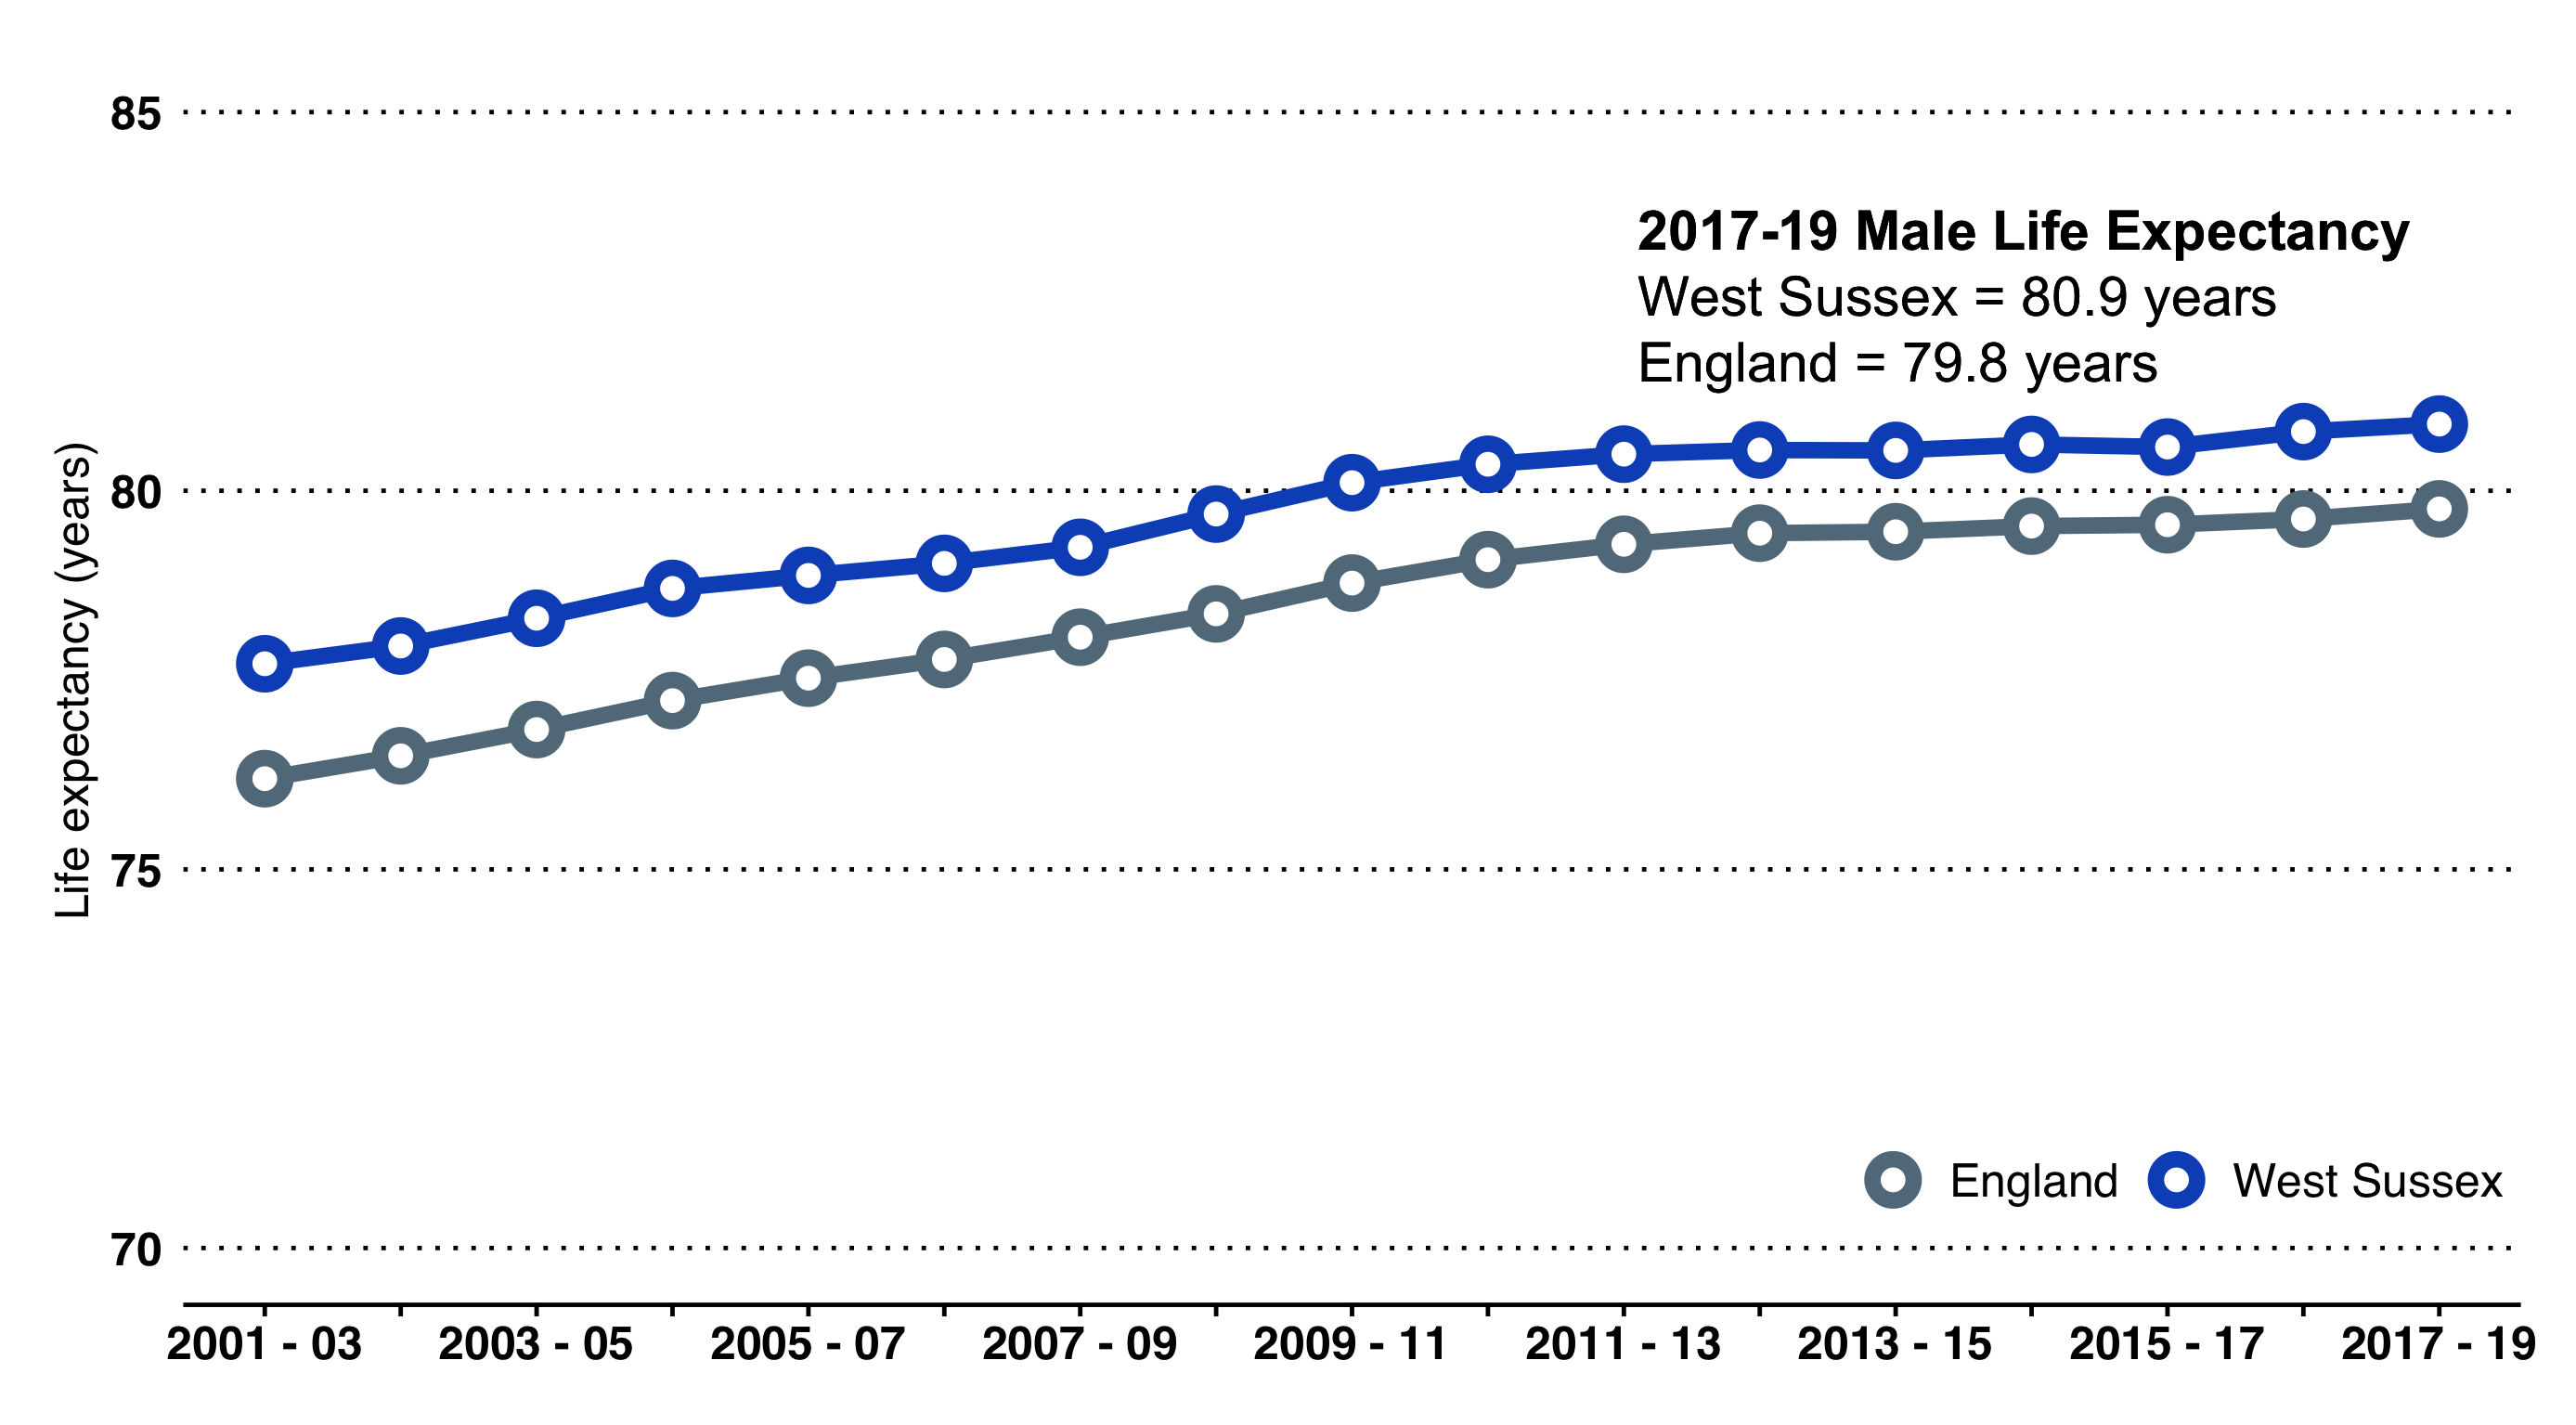
\includegraphics[width=\linewidth]{images/male_life_expectancy.png}
	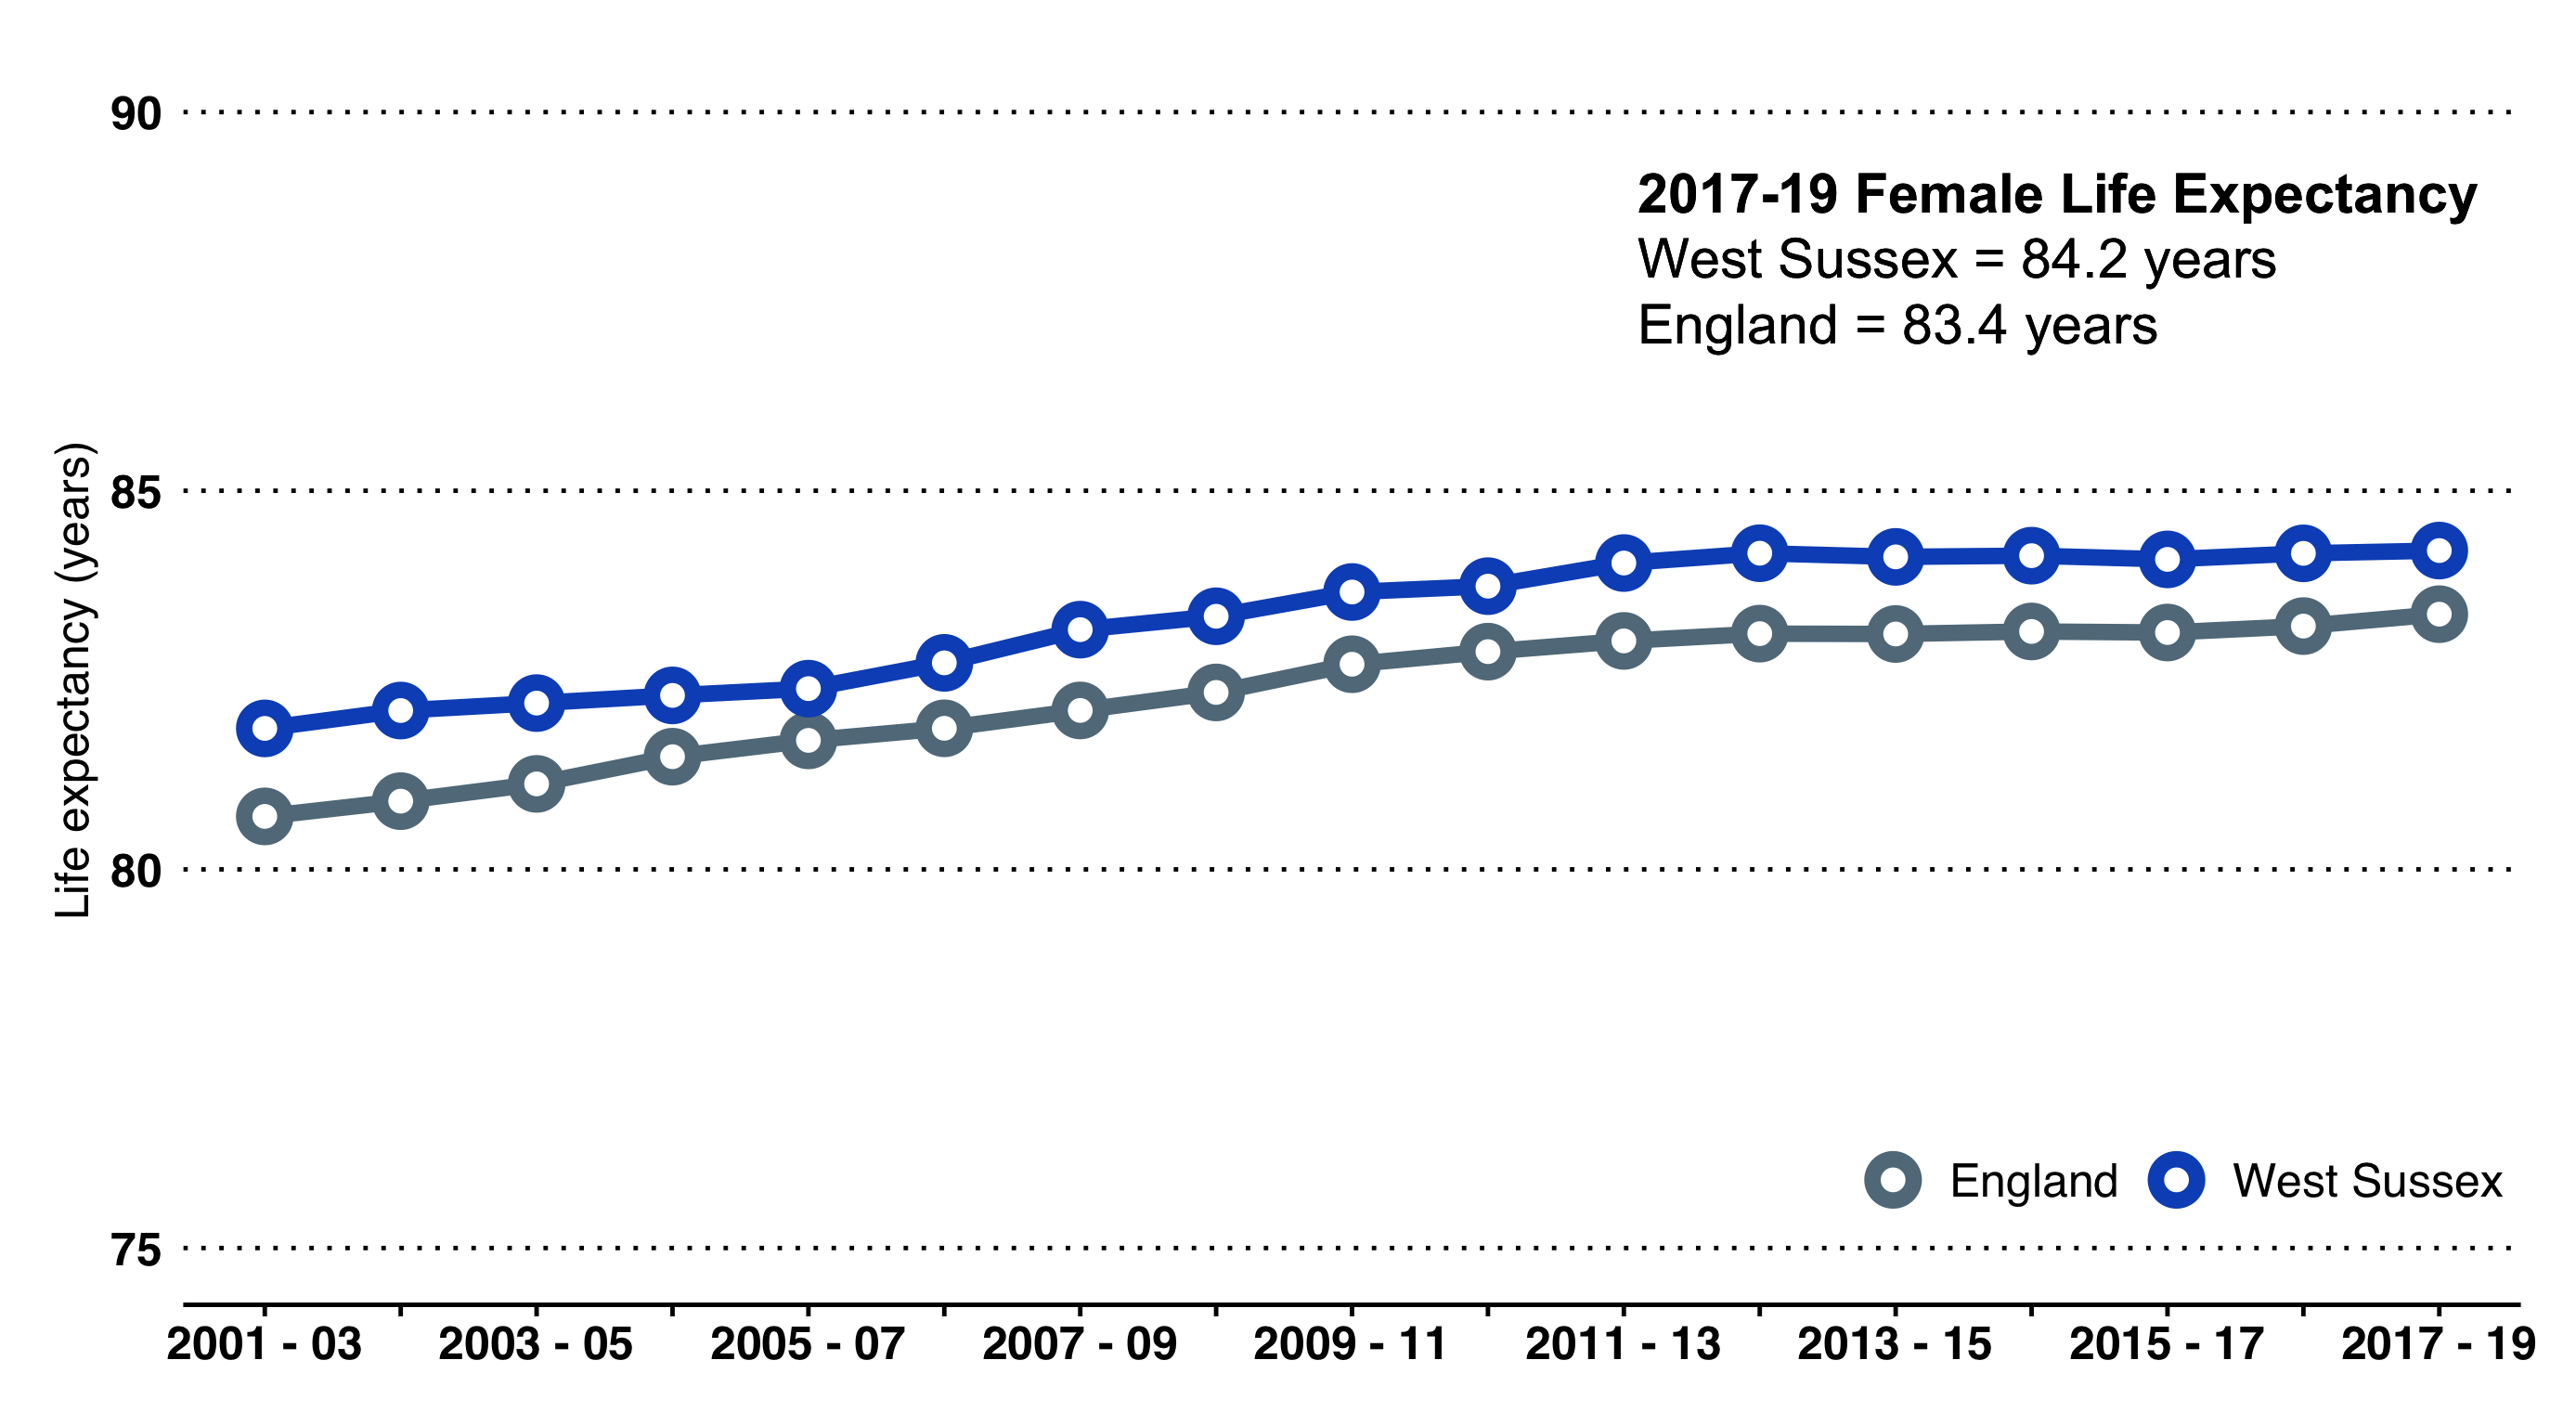
\includegraphics[width=\linewidth]{images/female_life_expectancy.png}
	\label{fig:life_exp}
\end{figure}

Difference in years of life expectancy between the least deprived and most deprived areas in West Sussex (2017-2019): Males from the most deprived area live on average 7 years fewer than males from the least deprived areas. Females from the most deprived areas live on average 6 years fewer than females from the least deprived areas.

For both men and women, circulatory causes (including stroke and heart disease) account for approximately a quarter of the difference, with cancers a further fifth of the difference\footnote{Note from OHID: Circulatory causes include heart disease and stroke}.

\begin{figure}[htp]
    \caption{Life expectancy gap between the most deprived quintile and least deprived quintile of West Sussex, by broad cause of death, 2015-17}
    \centering
	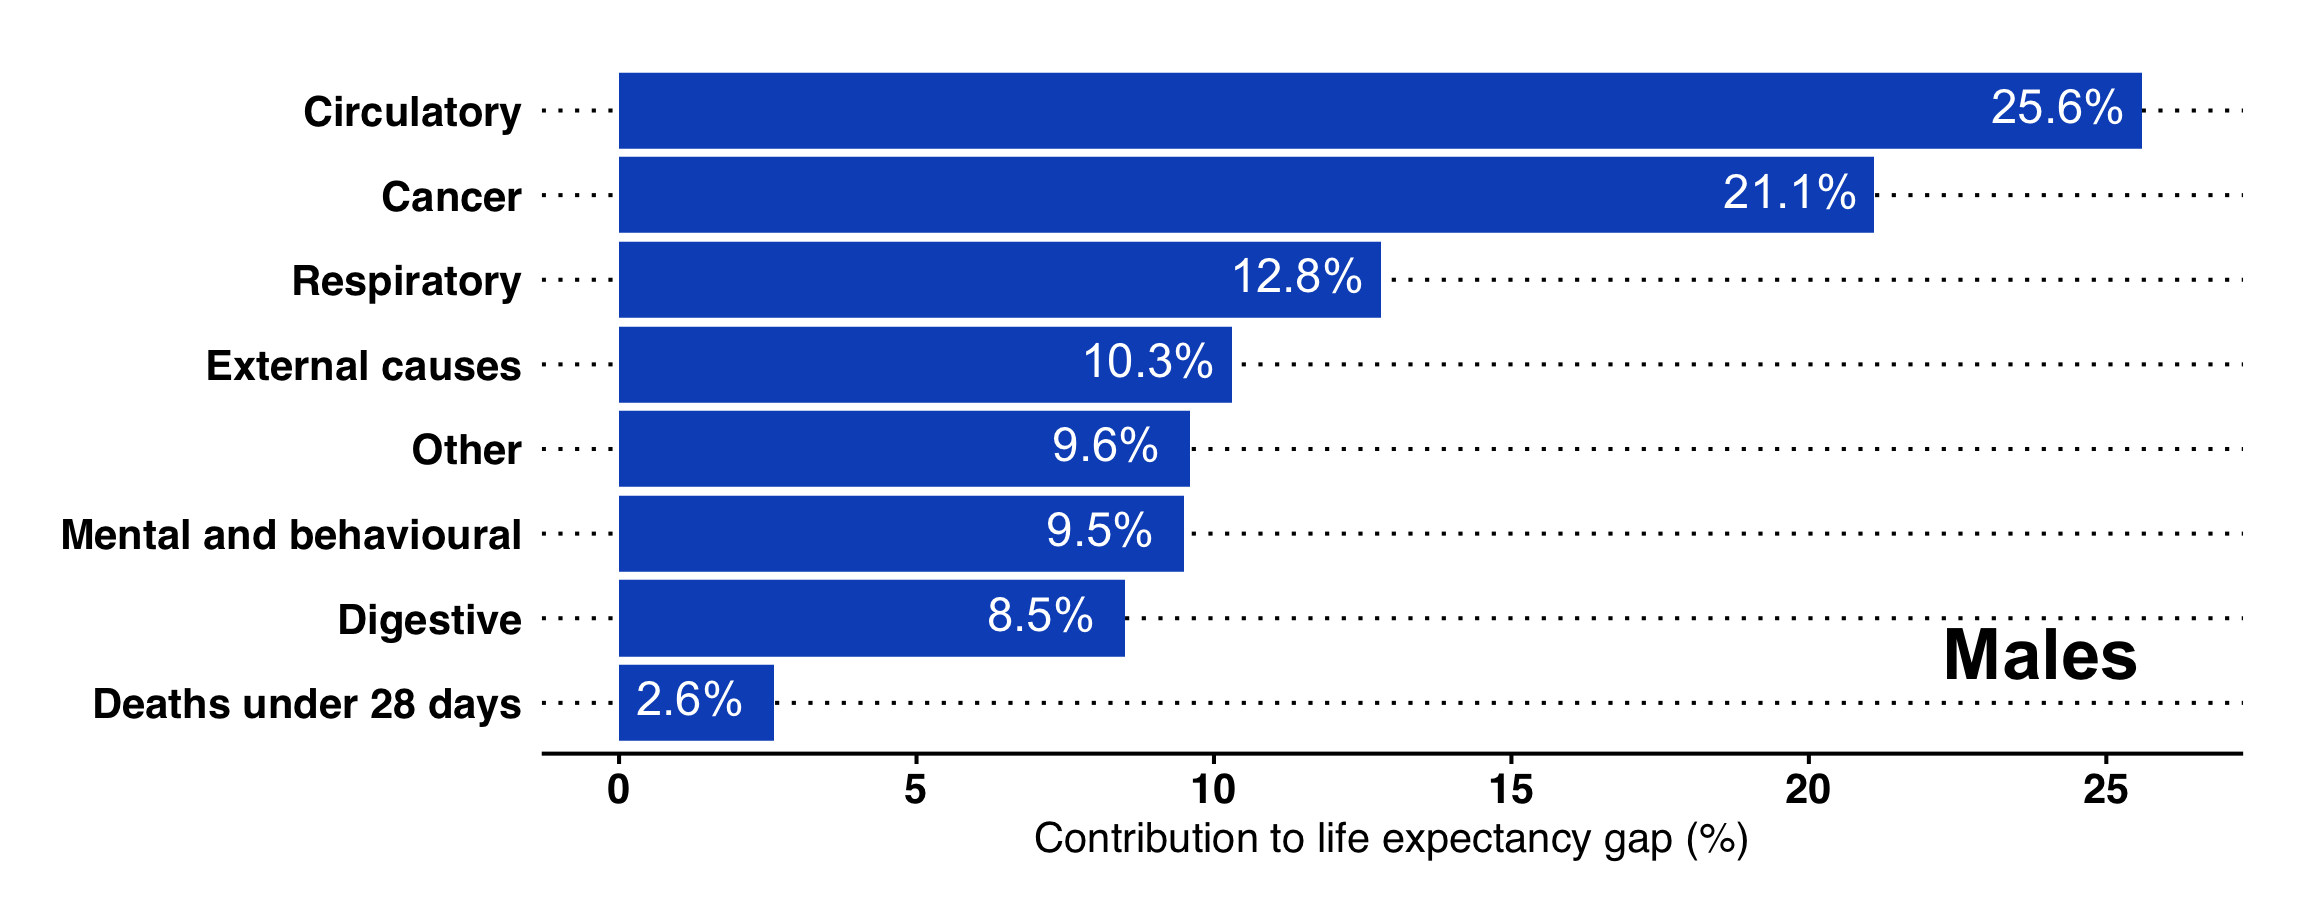
\includegraphics[width=\linewidth]{images/male_life_expectancy_gap.png}
	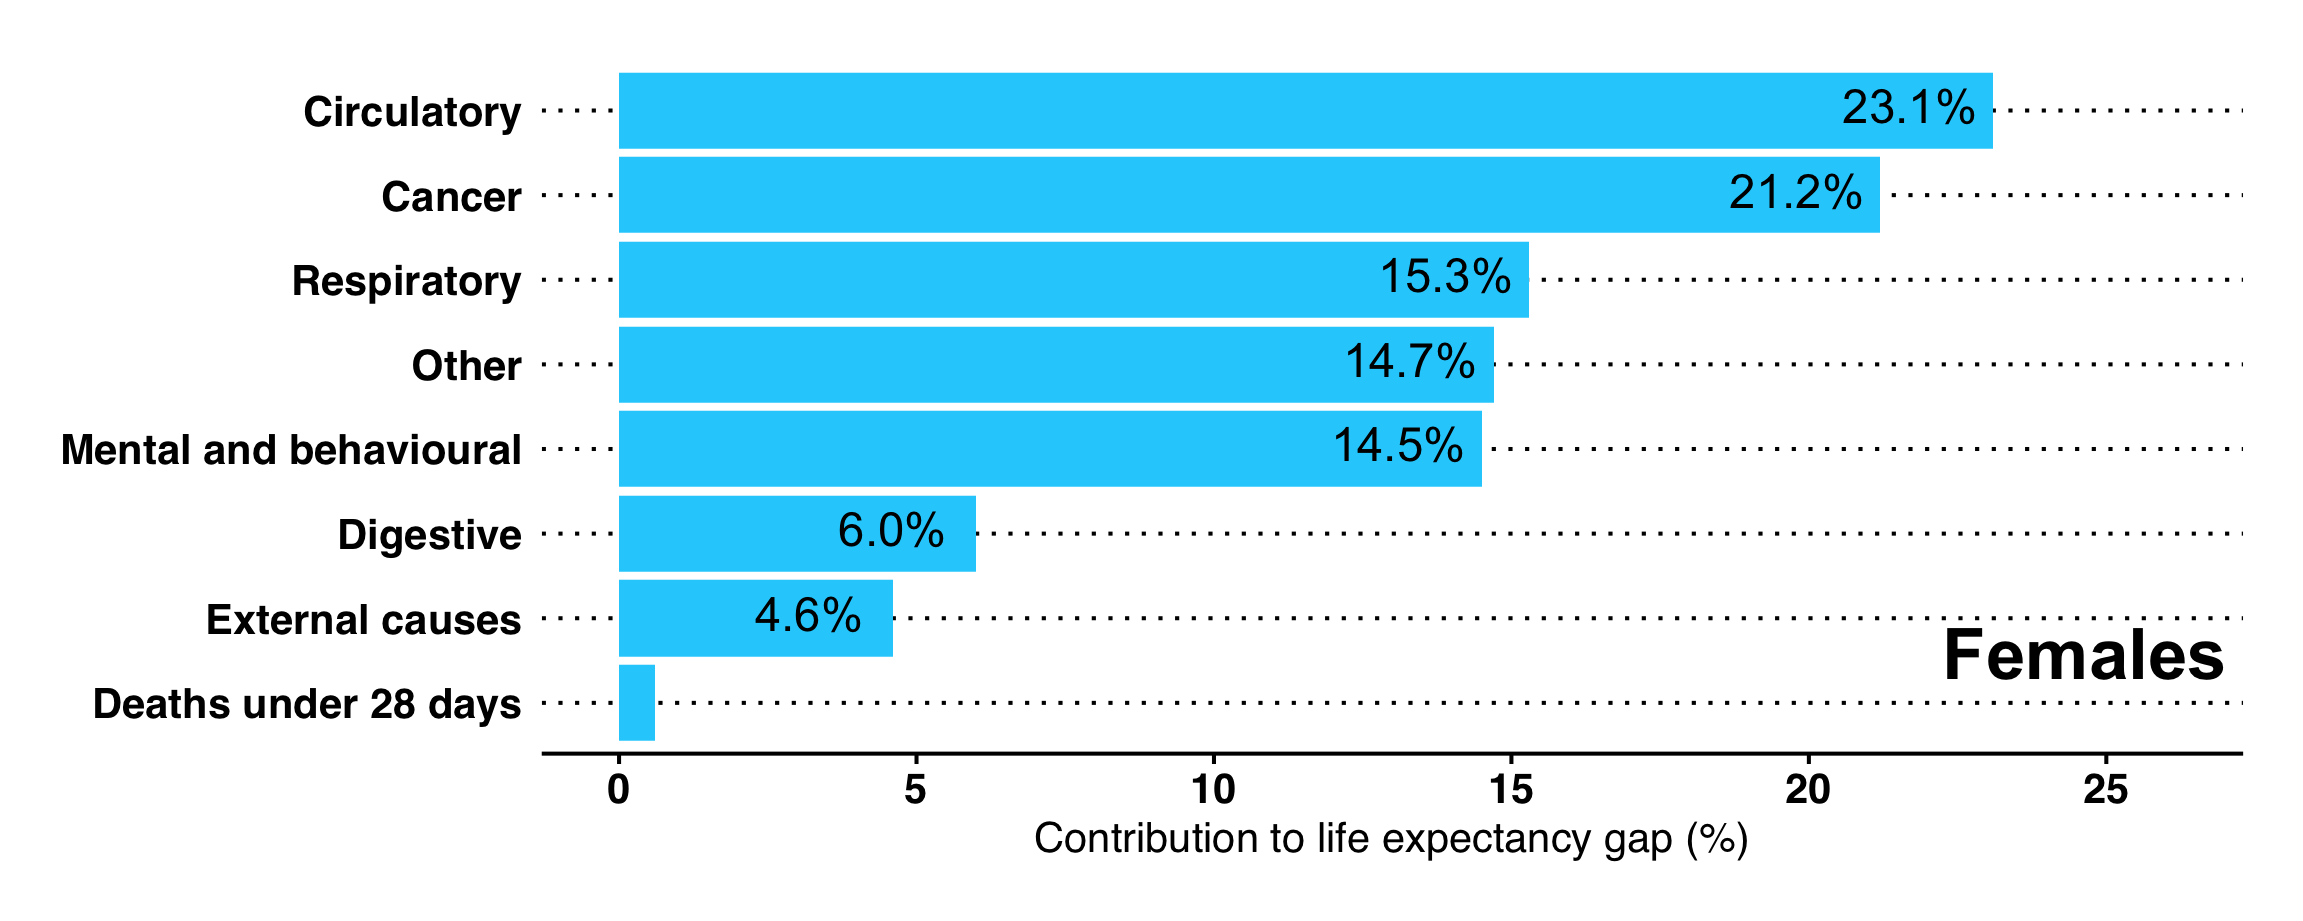
\includegraphics[width=\linewidth]{images/female_life_expectancy_gap.png}
	\label{fig:life_exp_gap}
\end{figure}

Respiratory includes flu, pneumonia, and chronic obstructive respiratory disease. Digestive includes alcohol-related conditions such as chronic liver disease and cirrhosis. External includes deaths from injury, poisoning and suicide. Mental and behavioural includes dementia and Alzheimer's disease. Percentages may not sum to 100 due to rounding.

PHE publish a segmentation tool to examine differences in life expectancy. Data are available at lower tier LA level \url{https://connect.healthdatainsight.org.uk/health_inequalities/segment_tool/}.

% \subsection{A focus on Social Mobility}
% \todo[inline]{This hasn't changed since last JSNA Summary (I think) so probably not worth repeating it, at least not in full.}
% The issue of social mobility has increased in prominence in recent years. In 2016, the Social Mobility Commission published data and ranked local authorities in terms of social mobility. The commission used a life stage approach looking at measures in the early years, school days, youth and adulthood. All 324 lower tier and unitary authorities were ranked, with the top 20\% performing areas, where social mobility opportunities were judged to be good, referred to as "hot spots" and the bottom 20\% of authorities, where opportunities are judged to be poor, as "cold spots". A summary is shown over the next two pages; the full briefing is available on the JSNA website. Contact Dr Verity Pinkney (\url{verity.pinkney@westsussex.gov.uk}) for further information.

% \paragraph{Key Points} Social mobility is about ensuring that young people have the same opportunities to succeed in life regardless of who they are or where they live. The social mobility index published by the Government\footnote{Note: This index was published in 2017 and some indicators will have changed since. The full report further explains the indicators behind the index. \url{https://www.gov.uk/government/publications/state-of-the-nation-2017}} looked at 16 key performance indicators which span our early years through to our working lives. This overall aim of the report was to answer the question: "What are the differences between local areas in the chances that a child from a disadvantaged socioeconomic background has of doing well as an adult?" There is a stark divide between London and the rest of the country, with nearly two-thirds of social mobility hotspots found in the capital. Arun, Chichester and Crawley were identified as social mobility cold spots on the overall index. Crawley was among the bottom 10\% of areas in England. Mid Sussex was the highest performer in West Sussex and was ranked 75th of the 324 local authorities in England.

% \paragraph{Younger people} Whilst the South East was the top performing region for early years, none of the local authorities in West Sussex were hotspots for this early age group and Chichester was a cold spot. Four local authorities in West Sussex were cold spots on the school age index. Crawley was the seventh worst in the country for school age. Of English local authorities, Crawley had the lowest proportion of children eligible for Free School Meals attending primary schools rated "good" or "outstanding" by OFSTED. Crawley was also identified as a cold spot for the youth index. Adults Horsham and Mid Sussex were hotspots on the adulthood index; this was due to high home ownership and fewer unskilled, low-paid jobs. Arun was the only local authority in West Sussex that was identified as a cold spot for adulthood.

% \paragraph{Crawley in Geographical Context - comparing Crawley with authorities bordering the M25} Crawley has a lot of assets, high employment and is close to London, yet it ranks low in terms of social mobility and now has areas ranked within the most deprived in the country. To understand Crawley in a wider geographic context, instead of comparing Crawley with the other West Sussex areas, we have looked at Crawley in context with 25 local authorities just outside the M25 (as a proxy for commuter belt areas), and deprivation relation to education and skills.

% This boxplot shows the ranks of small areas (LSOAs) within Crawley and 25 local authorities close to the M25, relating to education (KS2, KS4 and progression to higher education). A low rank means deprived, high rank means less deprived. In terms of education, Crawley is more deprived than the other authorities, with few areas within the town ranking in the less deprived deciles of the index of deprivation.

% FIGURE: Boxplot with ranks of small areas (LSOAs) within Crawley and 25 local authorities close to the M25, relating to education (KS2, KS4 and progression to higher education).

% \todo[inline]{Had a section here on the ICS - not sure now though}

%\subsection{An update on the ICS}

%How the primary care networks and clinical commissioning groups now slot in to the ICS picture.

%Website needs new single CCG profiles to replace the three former footprints.

%Do we want to have a subsection on pharmacies, perhaps in reference to Covid and vaccination?

%------------------------------------------------